\documentclass{article} 
\usepackage[utf8]{inputenc}
\usepackage[paperwidth=8.5in,paperheight=11in]{geometry}
%\usepackage[paperwidth=8.5in,paperheight=14.2885in]{geometry}
\geometry{left=2cm, right=2cm, top=2cm, bottom=2cm}
% Include the listings package for syntax highlighting
\usepackage{listingsutf8}
% Optional: include the xcolor package for more advanced color definitions
\usepackage[dvipsnames]{xcolor} 
\usepackage{multicol}  
\usepackage{amssymb,
			amsmath} 
\usepackage{dutchcal}
\usepackage{qlanth} 
% \usepackage{qlanthextras}
\usepackage{scalerel}
\usepackage{mdframed}
\usepackage{pgffor}
\usepackage{lmodern}
\usepackage[htt]{hyphenat} %Enable hythenation of TT text:
\usepackage[backend=bibtex,style=alphabetic]{biblatex}
\addbibresource{qlanth.bib} 
\newcommand{\codetext}[1]{{\color{BlueViolet} \texttt{#1}}} 
% Listing configuration
\lstset{   
    language=Mathematica,                   % Set your language (you can change the language for each code-block optionally)
    basicstyle=\ttfamily\color{darkgray}\small,       % The size of the fonts that are used for the code
    literate=
        {\\[Alpha]}{{$\alpha$}}{1}
        {\\[Beta]}{{$\beta$}}{1}
        {\\[Gamma]}{{$\gamma$}}{1}
        {\\[Zeta]}{{$\zeta$}}{1}
        {\\[VerticalSeparator]}{|}{1}
        ,  
    keywordstyle=\color{blue},        % Keyword style
    stringstyle=\color{OliveGreen},        % String literal style
    commentstyle=\color{cyan},        % Comment style
    morecomment=[l][\color{magenta}]{\#},
    breakatwhitespace=false,          % Sets if automatic breaks should only happen at whitespace
    breaklines=true,                  % Sets automatic line breaking
    captionpos=b,                     % Sets the caption-position to bottom
    keepspaces=true,                  % Keeps spaces in text, useful for keeping indentation of code (possibly needs columns=flexible)
    showspaces=false,                 % Show spaces everywhere adding particular underscores; it overrides 'showstringspaces'
    showstringspaces=false,           % Underline spaces within strings only
    showtabs=false,                   % Show tabs within strings adding particular underscores
    tabsize=2,                        % Sets default tabsize to 2 spaces
    frame=single,                     % Adds a frame around the code
    numbers=left,                     % Where to put the line-numbers; possible values are (none, left, right)
    numberstyle=\tiny\color{gray},    % Style used for line-numbers
    stepnumber=1,                     % Step between two line-numbers. If it's 1, each line will be numbered
    numbersep=5pt,                    % How far the line-numbers are from the code
    xleftmargin=0.8cm,                % Margin from left
    xrightmargin=0.3cm              % Margin from right
}
\usepackage[colorlinks=true, citecolor=blue, linkcolor=blue, urlcolor=cyan]{hyperref}

\usepackage{fancyhdr}
\pagestyle{fancy}
\fancyhf{}
\renewcommand{\headrulewidth}{0pt} % Optional: Removes the header rule
\cfoot{\hyperlink{toc}{\thepage}}

\begin{document} 

\begin{titlepage} % Start of the title page
    \centering
    \vspace*{\fill}
    
    % Include the image
    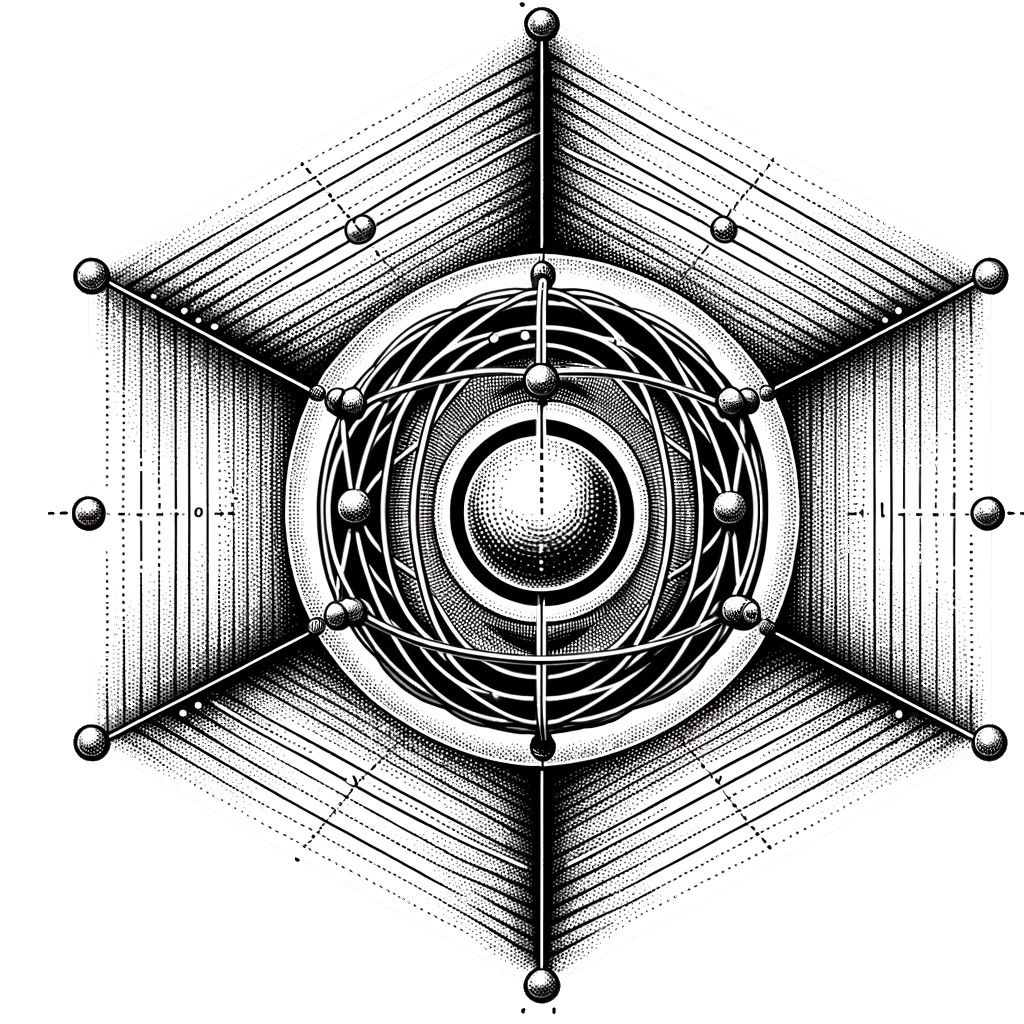
\includegraphics[width=0.6\textwidth]{ion_in_lattice.jpg} % Adjust the size as needed
    \vspace*{1cm} % More vertical space
    
    % Software name
    {\Large\qlanth}\\
    \vspace*{0.5cm}
    {\large version $\ket{\alpha}^{(5)}$}\\
    \vspace*{2cm}
    
    % Additional information
    {\large Juan David Lizarazo Ferro}\\
    {\large \& Christopher Dodson}\\
    \vspace{0.5cm}
    {\large Under the advisory of Dr. Rashid Zia}\\
    \vspace*{\fill}
\end{titlepage}

\newpage

\

\cleardoublepage

\hypertarget{toc}{}

\vspace*{\fill}

\tableofcontents

\vspace*{\fill}

\newpage

\qlanth is a tool that can be used to estimate the electronic structure of lanthanide ions in crystals. For this purpose it uses a single configuration description and a corresponding effective Hamiltonian. This Hamiltonian aims to describe the observed properties of ions embedded in solids in a picture that imagines them as free-ions but modified by the influence of the lattice in which they find themselves in.

This picture is one that developed and mostly matured in the second half of the last century by the efforts of Giulio Racah, Brian Judd, Hannah Crosswhite, Robert Cowan, Michael Reid, Bill Carnall, Clyde Morrison, Richard Leavitt, Brian Wybourne, and Katherine Rajnak among others. The goal of this tool is to provide a modern implementation of the methods that resulted from their work. This code is written in Wolfram language.

\qlanth also includes data that might be of use to those interested in the single-configuration description of lanthanide ions, separate to their specific use in this code. These data include the \cfps (as calculated by Velkov and parsed here), and reduced matrix elements for all the operators in the effective Hamiltonian. These are provided as standard Mathematica associations that should be simple to use elsewhere.

The included Mathematica notebook \codetext{qlanth.nb} has examples of the capabilities that this tool offers, and the \codetext{/examples} folder includes a series of notebooks for most of the trivalent lanthanide ions in lanthanum fluoride. \LaFthree is remarkable in that it was one of the systems in which a systematic study \cite{carnall_systematic_1989} of all of the trivalent lanthanide ions were studied. 

This code was originally authored by Christopher Dodson and Rashid Zia for their research into magnetic dipole transitions in lanthanide ions \cite{dodson_magnetic_2012}. Here it has been modified and rewritten by David Lizarazo. It has also benefited from conversations with Tharnier Puel at the University of Iowa.

This document has 12 sections. \textbf{Section 1} explains the details of the basis in which the Hamiltonian is evaluated. \textbf{Section 2} provides a brief explanation of the \cfps. \textbf{Section 3} explains how the Hamiltonian is put together by first having calculated ``$JJ'$ blocks''. \textbf{Section 4} is dedicated to a theoretical exposition of the effective Hamiltonian with subsections for each of the terms that it contains. \textbf{Section 5} is about the calculation of magnetic dipole transitions. \textbf{Sections 6 and 8} list additional data included in \qlanth. \textbf{Section 7} has additional information about data fitting.  \textbf{Section 9} has a brief comment on units. \textbf{Sections 9 and 10} include a summary of notation and definitions use throughout this document. Finally, \textbf{section 12} contains a printout of the code included in \qlanth.


\section{The $\LSJMbasis$ Basis}

The basis used in \qlanth is the $\LSJMbasis$ basis. As such the basis vectors are common eigenvectors of the operators $\op{L}^2$, $\op{S}^2$, $\op{J}^2$, and $\op{J}_z$. The LS terms allowed in each configuration $\forb^\numE$ are obtained from tables that originate from the original work by Nielson and Koster \cite{nielson_spectroscopic_1963}. In \qlanth these are parsed from the file \codetext{B1F\_ALL.TXT} which is part of the doctoral research of Dobromir Velkov \cite{velkov_multi-electron_2000} in which he recomputed \cfps under the advisory of Brian Judd. 

One of the facts that have to be accounted for in a basis that uses L and S as quantum numbers, is that there might be several linearly independent path to couple the electron spin and orbital momenta to add up to given total $L$ and total $S$. For this reason additional labels are necessary to distinguish between these different terms. The simplest way of doing this dates back to the tables of Nielson and Koster \cite{nielson_spectroscopic_1963}, and consists in assigning consecutive integers to degenerate LS terms, with no specific role given to them, except that of discriminating between different degenerate terms. 
 
The following are all the LS terms in the $\forb^{\numE}$ configurations. In the notation used the superscript index before the letter notes the spin multiplicity $2S+1$, the roman letter indicating the value of $L$ in spectroscopic notation ($S\!\!\rightarrow\!\!1, P\!\!\rightarrow\!\!2, D\!\!\rightarrow\!\!3, F\!\!\rightarrow\!\!4, G\!\!\rightarrow\!\!5, H\!\!\rightarrow\!\!6, I\!\!\rightarrow\!\!7, K\!\!\rightarrow\!\!8, L\!\!\rightarrow\!\!9, M\!\!\rightarrow\!\!10, N\!\!\rightarrow\!\!11, O\!\!\rightarrow\!\!12, Q\!\!\rightarrow\!\!3, R\!\!\rightarrow\!\!14, T\!\!\rightarrow\!\!15, U\!\!\rightarrow\!\!16, V\!\!\rightarrow\!\!17$), and the final integer (if present) is the label that discriminates between several degenerate LS. This index we frequently label in the equations contained in this document with the greek letter $\alpha$.

\begin{mdframed}
\begin{center}
$\forb^{0}$

(1 LS term)
\vspace{0.25cm}
\hrule
\vspace{0.25cm}

$\LSterm{1}{S}$
\end{center}
\end{mdframed}

\begin{mdframed}
\begin{center}
$\forb^{1}$

(1 LS term)
\vspace{0.25cm}
\hrule
\vspace{0.25cm}

$\LSterm{2}{F}$
\end{center}
\end{mdframed}

\begin{mdframed}
\begin{center}
$\forb^{2}$

(7 LS terms)
\vspace{0.25cm}
\hrule
\vspace{0.25cm}

$\LSterm{3}{P}$, $\LSterm{3}{F}$, $\LSterm{3}{H}$, $\LSterm{1}{S}$, $\LSterm{1}{D}$, $\LSterm{1}{G}$, $\LSterm{1}{I}$
\end{center}
\end{mdframed}

\begin{mdframed}
\begin{center}
$\forb^{3}$

(17 LS terms)
\vspace{0.25cm}
\hrule
\vspace{0.25cm}

$\LSterm{4}{S}$, $\LSterm{4}{D}$, $\LSterm{4}{F}$, $\LSterm{4}{G}$, $\LSterm{4}{I}$, $\LSterm{2}{P}$, $\LSterm{2}{D1}$, $\LSterm{2}{D2}$, $\LSterm{2}{F1}$, $\LSterm{2}{F2}$, $\LSterm{2}{G1}$, $\LSterm{2}{G2}$, $\LSterm{2}{H1}$, $\LSterm{2}{H2}$, $\LSterm{2}{I}$, $\LSterm{2}{K}$, $\LSterm{2}{L}$
\end{center}
\end{mdframed}

\begin{mdframed}
\begin{center}
$\forb^{4}$

(47 LS terms)
\vspace{0.25cm}
\hrule
\vspace{0.25cm}

$\LSterm{5}{S}$, $\LSterm{5}{D}$, $\LSterm{5}{F}$, $\LSterm{5}{G}$, $\LSterm{5}{I}$, $\LSterm{3}{P1}$, $\LSterm{3}{P2}$, $\LSterm{3}{P3}$, $\LSterm{3}{D1}$, $\LSterm{3}{D2}$, $\LSterm{3}{F1}$, $\LSterm{3}{F2}$, $\LSterm{3}{F3}$, $\LSterm{3}{F4}$, $\LSterm{3}{G1}$, $\LSterm{3}{G2}$, $\LSterm{3}{G3}$, $\LSterm{3}{H1}$, $\LSterm{3}{H2}$, $\LSterm{3}{H3}$, $\LSterm{3}{H4}$, $\LSterm{3}{I1}$, $\LSterm{3}{I2}$, $\LSterm{3}{K1}$, $\LSterm{3}{K2}$, $\LSterm{3}{L}$, $\LSterm{3}{M}$, $\LSterm{1}{S1}$, $\LSterm{1}{S2}$, $\LSterm{1}{D1}$, $\LSterm{1}{D2}$, $\LSterm{1}{D3}$, $\LSterm{1}{D4}$, $\LSterm{1}{F}$, $\LSterm{1}{G1}$, $\LSterm{1}{G2}$, $\LSterm{1}{G3}$, $\LSterm{1}{G4}$, $\LSterm{1}{H1}$, $\LSterm{1}{H2}$, $\LSterm{1}{I1}$, $\LSterm{1}{I2}$, $\LSterm{1}{I3}$, $\LSterm{1}{K}$, $\LSterm{1}{L1}$, $\LSterm{1}{L2}$, $\LSterm{1}{N}$
\end{center}
\end{mdframed}

\begin{mdframed}
\begin{center}
$\forb^{5}$

(73 LS terms)
\vspace{0.25cm}
\hrule
\vspace{0.25cm}

$\LSterm{6}{P}$, $\LSterm{6}{F}$, $\LSterm{6}{H}$, $\LSterm{4}{S}$, $\LSterm{4}{P1}$, $\LSterm{4}{P2}$, $\LSterm{4}{D1}$, $\LSterm{4}{D2}$, $\LSterm{4}{D3}$, $\LSterm{4}{F1}$, $\LSterm{4}{F2}$, $\LSterm{4}{F3}$, $\LSterm{4}{F4}$, $\LSterm{4}{G1}$, $\LSterm{4}{G2}$, $\LSterm{4}{G3}$, $\LSterm{4}{G4}$, $\LSterm{4}{H1}$, $\LSterm{4}{H2}$, $\LSterm{4}{H3}$, $\LSterm{4}{I1}$, $\LSterm{4}{I2}$, $\LSterm{4}{I3}$, $\LSterm{4}{K1}$, $\LSterm{4}{K2}$, $\LSterm{4}{L}$, $\LSterm{4}{M}$, $\LSterm{2}{P1}$, $\LSterm{2}{P2}$, $\LSterm{2}{P3}$, $\LSterm{2}{P4}$, $\LSterm{2}{D1}$, $\LSterm{2}{D2}$, $\LSterm{2}{D3}$, $\LSterm{2}{D4}$, $\LSterm{2}{D5}$, $\LSterm{2}{F1}$, $\LSterm{2}{F2}$, $\LSterm{2}{F3}$, $\LSterm{2}{F4}$, $\LSterm{2}{F5}$, $\LSterm{2}{F6}$, $\LSterm{2}{F7}$, $\LSterm{2}{G1}$, $\LSterm{2}{G2}$, $\LSterm{2}{G3}$, $\LSterm{2}{G4}$, $\LSterm{2}{G5}$, $\LSterm{2}{G6}$, $\LSterm{2}{H1}$, $\LSterm{2}{H2}$, $\LSterm{2}{H3}$, $\LSterm{2}{H4}$, $\LSterm{2}{H5}$, $\LSterm{2}{H6}$, $\LSterm{2}{H7}$, $\LSterm{2}{I1}$, $\LSterm{2}{I2}$, $\LSterm{2}{I3}$, $\LSterm{2}{I4}$, $\LSterm{2}{I5}$, $\LSterm{2}{K1}$, $\LSterm{2}{K2}$, $\LSterm{2}{K3}$, $\LSterm{2}{K4}$, $\LSterm{2}{K5}$, $\LSterm{2}{L1}$, $\LSterm{2}{L2}$, $\LSterm{2}{L3}$, $\LSterm{2}{M1}$, $\LSterm{2}{M2}$, $\LSterm{2}{N}$, $\LSterm{2}{O}$
\end{center}
\end{mdframed}

\begin{mdframed}
\begin{center}
$\forb^{6}$

(119 LS terms)
\vspace{0.25cm}
\hrule
\vspace{0.25cm}

$\LSterm{7}{F}$, $\LSterm{5}{S}$, $\LSterm{5}{P}$, $\LSterm{5}{D1}$, $\LSterm{5}{D2}$, $\LSterm{5}{D3}$, $\LSterm{5}{F1}$, $\LSterm{5}{F2}$, $\LSterm{5}{G1}$, $\LSterm{5}{G2}$, $\LSterm{5}{G3}$, $\LSterm{5}{H1}$, $\LSterm{5}{H2}$, $\LSterm{5}{I1}$, $\LSterm{5}{I2}$, $\LSterm{5}{K}$, $\LSterm{5}{L}$, $\LSterm{3}{P1}$, $\LSterm{3}{P2}$, $\LSterm{3}{P3}$, $\LSterm{3}{P4}$, $\LSterm{3}{P5}$, $\LSterm{3}{P6}$, $\LSterm{3}{D1}$, $\LSterm{3}{D2}$, $\LSterm{3}{D3}$, $\LSterm{3}{D4}$, $\LSterm{3}{D5}$, $\LSterm{3}{F1}$, $\LSterm{3}{F2}$, $\LSterm{3}{F3}$, $\LSterm{3}{F4}$, $\LSterm{3}{F5}$, $\LSterm{3}{F6}$, $\LSterm{3}{F7}$, $\LSterm{3}{F8}$, $\LSterm{3}{F9}$, $\LSterm{3}{G1}$, $\LSterm{3}{G2}$, $\LSterm{3}{G3}$, $\LSterm{3}{G4}$, $\LSterm{3}{G5}$, $\LSterm{3}{G6}$, $\LSterm{3}{G7}$, $\LSterm{3}{H1}$, $\LSterm{3}{H2}$, $\LSterm{3}{H3}$, $\LSterm{3}{H4}$, $\LSterm{3}{H5}$, $\LSterm{3}{H6}$, $\LSterm{3}{H7}$, $\LSterm{3}{H8}$, $\LSterm{3}{H9}$, $\LSterm{3}{I1}$, $\LSterm{3}{I2}$, $\LSterm{3}{I3}$, $\LSterm{3}{I4}$, $\LSterm{3}{I5}$, $\LSterm{3}{I6}$, $\LSterm{3}{K1}$, $\LSterm{3}{K2}$, $\LSterm{3}{K3}$, $\LSterm{3}{K4}$, $\LSterm{3}{K5}$, $\LSterm{3}{K6}$, $\LSterm{3}{L1}$, $\LSterm{3}{L2}$, $\LSterm{3}{L3}$, $\LSterm{3}{M1}$, $\LSterm{3}{M2}$, $\LSterm{3}{M3}$, $\LSterm{3}{N}$, $\LSterm{3}{O}$, $\LSterm{1}{S1}$, $\LSterm{1}{S2}$, $\LSterm{1}{S3}$, $\LSterm{1}{S4}$, $\LSterm{1}{P}$, $\LSterm{1}{D1}$, $\LSterm{1}{D2}$, $\LSterm{1}{D3}$, $\LSterm{1}{D4}$, $\LSterm{1}{D5}$, $\LSterm{1}{D6}$, $\LSterm{1}{F1}$, $\LSterm{1}{F2}$, $\LSterm{1}{F3}$, $\LSterm{1}{F4}$, $\LSterm{1}{G1}$, $\LSterm{1}{G2}$, $\LSterm{1}{G3}$, $\LSterm{1}{G4}$, $\LSterm{1}{G5}$, $\LSterm{1}{G6}$, $\LSterm{1}{G7}$, $\LSterm{1}{G8}$, $\LSterm{1}{H1}$, $\LSterm{1}{H2}$, $\LSterm{1}{H3}$, $\LSterm{1}{H4}$, $\LSterm{1}{I1}$, $\LSterm{1}{I2}$, $\LSterm{1}{I3}$, $\LSterm{1}{I4}$, $\LSterm{1}{I5}$, $\LSterm{1}{I6}$, $\LSterm{1}{I7}$, $\LSterm{1}{K1}$, $\LSterm{1}{K2}$, $\LSterm{1}{K3}$, $\LSterm{1}{L1}$, $\LSterm{1}{L2}$, $\LSterm{1}{L3}$, $\LSterm{1}{L4}$, $\LSterm{1}{M1}$, $\LSterm{1}{M2}$, $\LSterm{1}{N1}$, $\LSterm{1}{N2}$, $\LSterm{1}{Q}$
\end{center}
\end{mdframed}

\begin{mdframed}
\begin{center}
$\forb^{7}$

(119 LS terms)
\vspace{0.25cm}
\hrule
\vspace{0.25cm}

$\LSterm{8}{S}$, $\LSterm{6}{P}$, $\LSterm{6}{D}$, $\LSterm{6}{F}$, $\LSterm{6}{G}$, $\LSterm{6}{H}$, $\LSterm{6}{I}$, $\LSterm{4}{S1}$, $\LSterm{4}{S2}$, $\LSterm{4}{P1}$, $\LSterm{4}{P2}$, $\LSterm{4}{D1}$, $\LSterm{4}{D2}$, $\LSterm{4}{D3}$, $\LSterm{4}{D4}$, $\LSterm{4}{D5}$, $\LSterm{4}{D6}$, $\LSterm{4}{F1}$, $\LSterm{4}{F2}$, $\LSterm{4}{F3}$, $\LSterm{4}{F4}$, $\LSterm{4}{F5}$, $\LSterm{4}{G1}$, $\LSterm{4}{G2}$, $\LSterm{4}{G3}$, $\LSterm{4}{G4}$, $\LSterm{4}{G5}$, $\LSterm{4}{G6}$, $\LSterm{4}{G7}$, $\LSterm{4}{H1}$, $\LSterm{4}{H2}$, $\LSterm{4}{H3}$, $\LSterm{4}{H4}$, $\LSterm{4}{H5}$, $\LSterm{4}{I1}$, $\LSterm{4}{I2}$, $\LSterm{4}{I3}$, $\LSterm{4}{I4}$, $\LSterm{4}{I5}$, $\LSterm{4}{K1}$, $\LSterm{4}{K2}$, $\LSterm{4}{K3}$, $\LSterm{4}{L1}$, $\LSterm{4}{L2}$, $\LSterm{4}{L3}$, $\LSterm{4}{M}$, $\LSterm{4}{N}$, $\LSterm{2}{S1}$, $\LSterm{2}{S2}$, $\LSterm{2}{P1}$, $\LSterm{2}{P2}$, $\LSterm{2}{P3}$, $\LSterm{2}{P4}$, $\LSterm{2}{P5}$, $\LSterm{2}{D1}$, $\LSterm{2}{D2}$, $\LSterm{2}{D3}$, $\LSterm{2}{D4}$, $\LSterm{2}{D5}$, $\LSterm{2}{D6}$, $\LSterm{2}{D7}$, $\LSterm{2}{F1}$, $\LSterm{2}{F2}$, $\LSterm{2}{F3}$, $\LSterm{2}{F4}$, $\LSterm{2}{F5}$, $\LSterm{2}{F6}$, $\LSterm{2}{F7}$, $\LSterm{2}{F8}$, $\LSterm{2}{F9}$, $\LSterm{2}{F10}$, $\LSterm{2}{G1}$, $\LSterm{2}{G2}$, $\LSterm{2}{G3}$, $\LSterm{2}{G4}$, $\LSterm{2}{G5}$, $\LSterm{2}{G6}$, $\LSterm{2}{G7}$, $\LSterm{2}{G8}$, $\LSterm{2}{G9}$, $\LSterm{2}{G10}$, $\LSterm{2}{H1}$, $\LSterm{2}{H2}$, $\LSterm{2}{H3}$, $\LSterm{2}{H4}$, $\LSterm{2}{H5}$, $\LSterm{2}{H6}$, $\LSterm{2}{H7}$, $\LSterm{2}{H8}$, $\LSterm{2}{H9}$, $\LSterm{2}{I1}$, $\LSterm{2}{I2}$, $\LSterm{2}{I3}$, $\LSterm{2}{I4}$, $\LSterm{2}{I5}$, $\LSterm{2}{I6}$, $\LSterm{2}{I7}$, $\LSterm{2}{I8}$, $\LSterm{2}{I9}$, $\LSterm{2}{K1}$, $\LSterm{2}{K2}$, $\LSterm{2}{K3}$, $\LSterm{2}{K4}$, $\LSterm{2}{K5}$, $\LSterm{2}{K6}$, $\LSterm{2}{K7}$, $\LSterm{2}{L1}$, $\LSterm{2}{L2}$, $\LSterm{2}{L3}$, $\LSterm{2}{L4}$, $\LSterm{2}{L5}$, $\LSterm{2}{M1}$, $\LSterm{2}{M2}$, $\LSterm{2}{M3}$, $\LSterm{2}{M4}$, $\LSterm{2}{N1}$, $\LSterm{2}{N2}$, $\LSterm{2}{O}$, $\LSterm{2}{Q}$
\end{center}
\end{mdframed}

\begin{mdframed}
\begin{center}
$\forb^{8}$

(119 LS terms)
\vspace{0.25cm}
\hrule
\vspace{0.25cm}

$\LSterm{7}{F}$, $\LSterm{5}{S}$, $\LSterm{5}{P}$, $\LSterm{5}{D1}$, $\LSterm{5}{D2}$, $\LSterm{5}{D3}$, $\LSterm{5}{F1}$, $\LSterm{5}{F2}$, $\LSterm{5}{G1}$, $\LSterm{5}{G2}$, $\LSterm{5}{G3}$, $\LSterm{5}{H1}$, $\LSterm{5}{H2}$, $\LSterm{5}{I1}$, $\LSterm{5}{I2}$, $\LSterm{5}{K}$, $\LSterm{5}{L}$, $\LSterm{3}{P1}$, $\LSterm{3}{P2}$, $\LSterm{3}{P3}$, $\LSterm{3}{P4}$, $\LSterm{3}{P5}$, $\LSterm{3}{P6}$, $\LSterm{3}{D1}$, $\LSterm{3}{D2}$, $\LSterm{3}{D3}$, $\LSterm{3}{D4}$, $\LSterm{3}{D5}$, $\LSterm{3}{F1}$, $\LSterm{3}{F2}$, $\LSterm{3}{F3}$, $\LSterm{3}{F4}$, $\LSterm{3}{F5}$, $\LSterm{3}{F6}$, $\LSterm{3}{F7}$, $\LSterm{3}{F8}$, $\LSterm{3}{F9}$, $\LSterm{3}{G1}$, $\LSterm{3}{G2}$, $\LSterm{3}{G3}$, $\LSterm{3}{G4}$, $\LSterm{3}{G5}$, $\LSterm{3}{G6}$, $\LSterm{3}{G7}$, $\LSterm{3}{H1}$, $\LSterm{3}{H2}$, $\LSterm{3}{H3}$, $\LSterm{3}{H4}$, $\LSterm{3}{H5}$, $\LSterm{3}{H6}$, $\LSterm{3}{H7}$, $\LSterm{3}{H8}$, $\LSterm{3}{H9}$, $\LSterm{3}{I1}$, $\LSterm{3}{I2}$, $\LSterm{3}{I3}$, $\LSterm{3}{I4}$, $\LSterm{3}{I5}$, $\LSterm{3}{I6}$, $\LSterm{3}{K1}$, $\LSterm{3}{K2}$, $\LSterm{3}{K3}$, $\LSterm{3}{K4}$, $\LSterm{3}{K5}$, $\LSterm{3}{K6}$, $\LSterm{3}{L1}$, $\LSterm{3}{L2}$, $\LSterm{3}{L3}$, $\LSterm{3}{M1}$, $\LSterm{3}{M2}$, $\LSterm{3}{M3}$, $\LSterm{3}{N}$, $\LSterm{3}{O}$, $\LSterm{1}{S1}$, $\LSterm{1}{S2}$, $\LSterm{1}{S3}$, $\LSterm{1}{S4}$, $\LSterm{1}{P}$, $\LSterm{1}{D1}$, $\LSterm{1}{D2}$, $\LSterm{1}{D3}$, $\LSterm{1}{D4}$, $\LSterm{1}{D5}$, $\LSterm{1}{D6}$, $\LSterm{1}{F1}$, $\LSterm{1}{F2}$, $\LSterm{1}{F3}$, $\LSterm{1}{F4}$, $\LSterm{1}{G1}$, $\LSterm{1}{G2}$, $\LSterm{1}{G3}$, $\LSterm{1}{G4}$, $\LSterm{1}{G5}$, $\LSterm{1}{G6}$, $\LSterm{1}{G7}$, $\LSterm{1}{G8}$, $\LSterm{1}{H1}$, $\LSterm{1}{H2}$, $\LSterm{1}{H3}$, $\LSterm{1}{H4}$, $\LSterm{1}{I1}$, $\LSterm{1}{I2}$, $\LSterm{1}{I3}$, $\LSterm{1}{I4}$, $\LSterm{1}{I5}$, $\LSterm{1}{I6}$, $\LSterm{1}{I7}$, $\LSterm{1}{K1}$, $\LSterm{1}{K2}$, $\LSterm{1}{K3}$, $\LSterm{1}{L1}$, $\LSterm{1}{L2}$, $\LSterm{1}{L3}$, $\LSterm{1}{L4}$, $\LSterm{1}{M1}$, $\LSterm{1}{M2}$, $\LSterm{1}{N1}$, $\LSterm{1}{N2}$, $\LSterm{1}{Q}$
\end{center}
\end{mdframed}

\begin{mdframed}
\begin{center}
$\forb^{9}$

(73 LS terms)
\vspace{0.25cm}
\hrule
\vspace{0.25cm}

$\LSterm{6}{P}$, $\LSterm{6}{F}$, $\LSterm{6}{H}$, $\LSterm{4}{S}$, $\LSterm{4}{P1}$, $\LSterm{4}{P2}$, $\LSterm{4}{D1}$, $\LSterm{4}{D2}$, $\LSterm{4}{D3}$, $\LSterm{4}{F1}$, $\LSterm{4}{F2}$, $\LSterm{4}{F3}$, $\LSterm{4}{F4}$, $\LSterm{4}{G1}$, $\LSterm{4}{G2}$, $\LSterm{4}{G3}$, $\LSterm{4}{G4}$, $\LSterm{4}{H1}$, $\LSterm{4}{H2}$, $\LSterm{4}{H3}$, $\LSterm{4}{I1}$, $\LSterm{4}{I2}$, $\LSterm{4}{I3}$, $\LSterm{4}{K1}$, $\LSterm{4}{K2}$, $\LSterm{4}{L}$, $\LSterm{4}{M}$, $\LSterm{2}{P1}$, $\LSterm{2}{P2}$, $\LSterm{2}{P3}$, $\LSterm{2}{P4}$, $\LSterm{2}{D1}$, $\LSterm{2}{D2}$, $\LSterm{2}{D3}$, $\LSterm{2}{D4}$, $\LSterm{2}{D5}$, $\LSterm{2}{F1}$, $\LSterm{2}{F2}$, $\LSterm{2}{F3}$, $\LSterm{2}{F4}$, $\LSterm{2}{F5}$, $\LSterm{2}{F6}$, $\LSterm{2}{F7}$, $\LSterm{2}{G1}$, $\LSterm{2}{G2}$, $\LSterm{2}{G3}$, $\LSterm{2}{G4}$, $\LSterm{2}{G5}$, $\LSterm{2}{G6}$, $\LSterm{2}{H1}$, $\LSterm{2}{H2}$, $\LSterm{2}{H3}$, $\LSterm{2}{H4}$, $\LSterm{2}{H5}$, $\LSterm{2}{H6}$, $\LSterm{2}{H7}$, $\LSterm{2}{I1}$, $\LSterm{2}{I2}$, $\LSterm{2}{I3}$, $\LSterm{2}{I4}$, $\LSterm{2}{I5}$, $\LSterm{2}{K1}$, $\LSterm{2}{K2}$, $\LSterm{2}{K3}$, $\LSterm{2}{K4}$, $\LSterm{2}{K5}$, $\LSterm{2}{L1}$, $\LSterm{2}{L2}$, $\LSterm{2}{L3}$, $\LSterm{2}{M1}$, $\LSterm{2}{M2}$, $\LSterm{2}{N}$, $\LSterm{2}{O}$
\end{center}
\end{mdframed}

\begin{mdframed}
\begin{center}
$\forb^{10}$

(47 LS terms)
\vspace{0.25cm}
\hrule
\vspace{0.25cm}

$\LSterm{5}{S}$, $\LSterm{5}{D}$, $\LSterm{5}{F}$, $\LSterm{5}{G}$, $\LSterm{5}{I}$, $\LSterm{3}{P1}$, $\LSterm{3}{P2}$, $\LSterm{3}{P3}$, $\LSterm{3}{D1}$, $\LSterm{3}{D2}$, $\LSterm{3}{F1}$, $\LSterm{3}{F2}$, $\LSterm{3}{F3}$, $\LSterm{3}{F4}$, $\LSterm{3}{G1}$, $\LSterm{3}{G2}$, $\LSterm{3}{G3}$, $\LSterm{3}{H1}$, $\LSterm{3}{H2}$, $\LSterm{3}{H3}$, $\LSterm{3}{H4}$, $\LSterm{3}{I1}$, $\LSterm{3}{I2}$, $\LSterm{3}{K1}$, $\LSterm{3}{K2}$, $\LSterm{3}{L}$, $\LSterm{3}{M}$, $\LSterm{1}{S1}$, $\LSterm{1}{S2}$, $\LSterm{1}{D1}$, $\LSterm{1}{D2}$, $\LSterm{1}{D3}$, $\LSterm{1}{D4}$, $\LSterm{1}{F}$, $\LSterm{1}{G1}$, $\LSterm{1}{G2}$, $\LSterm{1}{G3}$, $\LSterm{1}{G4}$, $\LSterm{1}{H1}$, $\LSterm{1}{H2}$, $\LSterm{1}{I1}$, $\LSterm{1}{I2}$, $\LSterm{1}{I3}$, $\LSterm{1}{K}$, $\LSterm{1}{L1}$, $\LSterm{1}{L2}$, $\LSterm{1}{N}$
\end{center}
\end{mdframed}

\begin{mdframed}
\begin{center}
$\forb^{11}$

(17 LS terms)
\vspace{0.25cm}
\hrule
\vspace{0.25cm}

$\LSterm{4}{S}$, $\LSterm{4}{D}$, $\LSterm{4}{F}$, $\LSterm{4}{G}$, $\LSterm{4}{I}$, $\LSterm{2}{P}$, $\LSterm{2}{D1}$, $\LSterm{2}{D2}$, $\LSterm{2}{F1}$, $\LSterm{2}{F2}$, $\LSterm{2}{G1}$, $\LSterm{2}{G2}$, $\LSterm{2}{H1}$, $\LSterm{2}{H2}$, $\LSterm{2}{I}$, $\LSterm{2}{K}$, $\LSterm{2}{L}$
\end{center}
\end{mdframed}

\begin{mdframed}
\begin{center}
$\forb^{12}$

(7 LS terms)
\vspace{0.25cm}
\hrule
\vspace{0.25cm}

$\LSterm{3}{P}$, $\LSterm{3}{F}$, $\LSterm{3}{H}$, $\LSterm{1}{S}$, $\LSterm{1}{D}$, $\LSterm{1}{G}$, $\LSterm{1}{I}$
\end{center}
\end{mdframed}

\begin{mdframed}
\begin{center}
$\forb^{13}$

(1 LS term)
\vspace{0.25cm}
\hrule
\vspace{0.25cm}

$\LSterm{2}{F}$
\end{center}
\end{mdframed}

\begin{mdframed}
\begin{center}
$\forb^{14}$

(1 LS term)
\vspace{0.25cm}
\hrule
\vspace{0.25cm}

$\LSterm{1}{S}$
\end{center}
\end{mdframed}

   
 
In \qlanth these terms may be queried through the function \codetext{AllowedNKSLTerms}. 

\foreach \name in {AllowedNKSLTerms}{ 
        \lstinputlisting[language=Mathematica]{./fundefs/\name.tex}
    }

In addition to LS the basis vector are also specified by the total angular momentum $J$ (which may go from $\abs{L-S}$ to $\abs{L+S}$). Then for each $J$ there are $2J+1$ projections on the z-axis. For example, the ordered $\LSJMbasis$ basis for $\forb^2$ is the one below. Where the first element is the LS term given as a string, the second equal to $J$, and the third one equal to $\Msub{J}$.
 
\begin{mdframed}
\begin{center}
$(J=0)$


(2 kets)
\vspace{0.25cm}\hrule\vspace{0.25cm}
$\ket{\LSterm{3}{P},0,0}$, $\ket{\LSterm{1}{S},0,0}$
\end{center}
\end{mdframed}

\begin{mdframed}
\begin{center}
$(J=1)$


(3 kets)
\vspace{0.25cm}\hrule\vspace{0.25cm}
$\ket{\LSterm{3}{P},1,-1}$, $\ket{\LSterm{3}{P},1,0}$, $\ket{\LSterm{3}{P},1,1}$
\end{center}
\end{mdframed}

\begin{mdframed}
\begin{center}
$(J=2)$


(15 kets)
\vspace{0.25cm}\hrule\vspace{0.25cm}
$\ket{\LSterm{3}{P},2,-2}$, $\ket{\LSterm{3}{P},2,-1}$, $\ket{\LSterm{3}{P},2,0}$, $\ket{\LSterm{3}{P},2,1}$, $\ket{\LSterm{3}{P},2,2}$, $\ket{\LSterm{3}{F},2,-2}$, $\ket{\LSterm{3}{F},2,-1}$, $\ket{\LSterm{3}{F},2,0}$, $\ket{\LSterm{3}{F},2,1}$, $\ket{\LSterm{3}{F},2,2}$, $\ket{\LSterm{1}{D},2,-2}$, $\ket{\LSterm{1}{D},2,-1}$, $\ket{\LSterm{1}{D},2,0}$, $\ket{\LSterm{1}{D},2,1}$, $\ket{\LSterm{1}{D},2,2}$
\end{center}
\end{mdframed}

\begin{mdframed}
\begin{center}
$(J=3)$


(7 kets)
\vspace{0.25cm}\hrule\vspace{0.25cm}
$\ket{\LSterm{3}{F},3,-3}$, $\ket{\LSterm{3}{F},3,-2}$, $\ket{\LSterm{3}{F},3,-1}$, $\ket{\LSterm{3}{F},3,0}$, $\ket{\LSterm{3}{F},3,1}$, $\ket{\LSterm{3}{F},3,2}$, $\ket{\LSterm{3}{F},3,3}$
\end{center}
\end{mdframed}

\begin{mdframed}
\begin{center}
$(J=4)$


(27 kets)
\vspace{0.25cm}\hrule\vspace{0.25cm}
$\ket{\LSterm{3}{F},4,-4}$, $\ket{\LSterm{3}{F},4,-3}$, $\ket{\LSterm{3}{F},4,-2}$, $\ket{\LSterm{3}{F},4,-1}$, $\ket{\LSterm{3}{F},4,0}$, $\ket{\LSterm{3}{F},4,1}$, $\ket{\LSterm{3}{F},4,2}$, $\ket{\LSterm{3}{F},4,3}$, $\ket{\LSterm{3}{F},4,4}$, $\ket{\LSterm{3}{H},4,-4}$, $\ket{\LSterm{3}{H},4,-3}$, $\ket{\LSterm{3}{H},4,-2}$, $\ket{\LSterm{3}{H},4,-1}$, $\ket{\LSterm{3}{H},4,0}$, $\ket{\LSterm{3}{H},4,1}$, $\ket{\LSterm{3}{H},4,2}$, $\ket{\LSterm{3}{H},4,3}$, $\ket{\LSterm{3}{H},4,4}$, $\ket{\LSterm{1}{G},4,-4}$, $\ket{\LSterm{1}{G},4,-3}$, $\ket{\LSterm{1}{G},4,-2}$, $\ket{\LSterm{1}{G},4,-1}$, $\ket{\LSterm{1}{G},4,0}$, $\ket{\LSterm{1}{G},4,1}$, $\ket{\LSterm{1}{G},4,2}$, $\ket{\LSterm{1}{G},4,3}$, $\ket{\LSterm{1}{G},4,4}$
\end{center}
\end{mdframed}

\begin{mdframed}
\begin{center}
$(J=5)$


(11 kets)
\vspace{0.25cm}\hrule\vspace{0.25cm}
$\ket{\LSterm{3}{H},5,-5}$, $\ket{\LSterm{3}{H},5,-4}$, $\ket{\LSterm{3}{H},5,-3}$, $\ket{\LSterm{3}{H},5,-2}$, $\ket{\LSterm{3}{H},5,-1}$, $\ket{\LSterm{3}{H},5,0}$, $\ket{\LSterm{3}{H},5,1}$, $\ket{\LSterm{3}{H},5,2}$, $\ket{\LSterm{3}{H},5,3}$, $\ket{\LSterm{3}{H},5,4}$, $\ket{\LSterm{3}{H},5,5}$
\end{center}
\end{mdframed}

\begin{mdframed}
\begin{center}
$(J=6)$


(26 kets)
\vspace{0.25cm}\hrule\vspace{0.25cm}
$\ket{\LSterm{3}{H},6,-6}$, $\ket{\LSterm{3}{H},6,-5}$, $\ket{\LSterm{3}{H},6,-4}$, $\ket{\LSterm{3}{H},6,-3}$, $\ket{\LSterm{3}{H},6,-2}$, $\ket{\LSterm{3}{H},6,-1}$, $\ket{\LSterm{3}{H},6,0}$, $\ket{\LSterm{3}{H},6,1}$, $\ket{\LSterm{3}{H},6,2}$, $\ket{\LSterm{3}{H},6,3}$, $\ket{\LSterm{3}{H},6,4}$, $\ket{\LSterm{3}{H},6,5}$, $\ket{\LSterm{3}{H},6,6}$, $\ket{\LSterm{1}{I},6,-6}$, $\ket{\LSterm{1}{I},6,-5}$, $\ket{\LSterm{1}{I},6,-4}$, $\ket{\LSterm{1}{I},6,-3}$, $\ket{\LSterm{1}{I},6,-2}$, $\ket{\LSterm{1}{I},6,-1}$, $\ket{\LSterm{1}{I},6,0}$, $\ket{\LSterm{1}{I},6,1}$, $\ket{\LSterm{1}{I},6,2}$, $\ket{\LSterm{1}{I},6,3}$, $\ket{\LSterm{1}{I},6,4}$, $\ket{\LSterm{1}{I},6,5}$, $\ket{\LSterm{1}{I},6,6}$
\end{center}
\end{mdframed} 

The order above is exemplar of the ordering in the bases. Notice how the basis vectors are sorted in order of increasing $J$, so that for instance not all of the basis kets associated with the $\LSterm{3}{P}$ LS term are contiguous. Within each group for a given $J$ the basis kets are then ordered in decreasing $S$, then ordered in increasing $L$, and then according to $\Msub{J}$.

In \qlanth the ordered basis used for a given $\forb^\numE$ is provided by \codetext{BasisLSJMJ}. 

\lstinputlisting[language=Mathematica]{./fundefs/BasisLSJMJ.tex}

\subsection{More quantun numbers}

Besides using an integer that simply solves the problem of discriminating between degenerate $LS$ terms by enumerating them, it is also possible to add more useful labels that reflect additional symmetries that the f-electron wavefunctions find in the groups $\SO{7}$ and $\Gtwo$.

\subsubsection{Seniority $\senior$}

The seniority number connects different LS terms between configurations, so that a term below can be seen as the \textit{senior} of a term above. To determine the seniority of a given term in configuration $\forb^\numE$ one must first find the configuration $\forb^{\tilde{\numE}}$ in which this term appeared. For example $\forb^{5}$ contains six degenerate ${}^2G$ terms. The first time this term appeared was in $\forb^3$, where it had a degeneracy of 2. The 2 degenerate terms in $\forb^3$ would then both have a seniority of $\senior=3$ since they first appeared in $\forb^3$. In consequency two of the six degenerate terms in $\forb^5$ would have the same degeneracy those two in $\forb^3$, and are therefore linked to those previous two. The four remaining ones, are  considered to be \textit{born} in $\forb^5$, and therefore have a seniority $\senior=5$.

These rules seem to be ad-hoc, but they are useful in dealing with the degeneracies in the LS terms as the arrive going up the configurations.

There is, however, a much deeper meaning to the seniority number. It can be shown that the seniority number (more exactly a quantity related to it) is a sort of spin, a quasi-spin, where the spin projections along the `z-axis' correspond to different number of electrons in $\forb^\numE$ configurations. This is a consequence of the Pauli exclusion principle. It is also useful to relate matrix elements of operators in one configuration to those in another, through the use of the Wigner-Eckart theorem. This is an interesting an useful theoretical construct, but the method of fractional parentage (which is what is implemented in $\qlanth$ is well suited also, albeit being somewhat less parsimonious than what the quasi-spin view that seniority can provide. As such $\qlanth$ does not use the seniority numbers that are associated with each LS term.

\subsubsection{$\RacahU$ and $\RacahW$}

Much as $L$ tells us how a rotation acts on a $L$ wavefunction by mixing different $\Msub{L}$ components, these other two labels specify how the wavefunctions transform under the operations of these other two groups. The $\RacahW$ label determines how a wavefunction transforms under a rotation in 7-dimensional space, and $\RacahU$ how they transform under an operator of group $\Gtwo$. Without going into the group theoretical details, the irreducible representations of $\SO{7}$ can be represented by triples of integer numbers, and those of $\Gtwo$ as pairs of two integers.

In \qlanth the $\RacahW$ and $\RacahU$ are used in order to determine the matrix elements of the $\casimir{\SO{7}}$ and $\casimir{\Gtwo}$ operators.

\section{The \cfps}

In the 1920s and 1930s, when spectroscopic evidence was being studied to elucidate the principles of quantum mechanics, one conceptual tool that was put forward for the analysis of the complex spectra of ions \cite{bacher_atomic_1934} involved using the spectrum of an ion at one stage of ionization to understand another stage.  For instance, using the fourth spectrum of oxygen (OIV) in order to understand the third spectrum (OIII) of the same element. 

In 1943 Giulio Racah \cite{racah_theory_1943} provided a useful extension to this idea. In addition of using the energies of one spectrum to span the energies of another, Racah extended this idea to the wavefunctions themselves, such that from configuration $\forb^{\numE-1}$ one can create the wavefunctions for $\forb^{\numE-1}$ with all the required antisymmetry and normalization conditions. In this approach, a given \textit{daughter} term in $\forb^{\numE}$ has a number of \textit{parent} terms in $\forb^{\numE-1}$, with the \cfps determining how much of each parent is in the daughter as a sum over parents
\begin{equation}
\ket{\lorb^\numE \alpha LS} = 
	\sum_{\bar{\alpha}\bar{L}
		\bar{S}} 
		\underbracket{\cfp{\lorb^{\numE-1}\bar{\alpha}\bar{L}\bar{S}}
			{\lorb^{\numE}\alpha{LS}}}_
		{\substack{
            \text{How much of parent }\ket{\lorb^{\numE-1}\bar{\alpha}\bar{L}\bar{S}} \\
            \text{is in daughter}\ket{\lorb^{\numE}{\alpha}{L}{S}}
            }
        }
		\underbracket{\ket{\left(\lorb^{\numE-1}\bar{\alpha}\bar{L}\bar{S},\lorb\right)\alpha{LS}}}_
		{\substack{
            \text{Couple an additional $\lorb$} \\
            \text{to the parent }\ket{\lorb^{\numE-1}\bar{\alpha}\bar{L}\bar{S}}
            }
        }.
\end{equation}

More importantly for \qlanth, the \cfps can be used to evaluate matrix elements of operators, such as in \eqnref{eqn:reducedV1k}, \eqnref{eqn:three body escalator}, \eqnref{eqn:ReducedUk}, and \eqnref{double cfp escalator}. These formulas realize a convenient calculation advantage: if one knows matrix elements in one configuration, then one can immediately calculate them in any other configuration.

In principle all the data that is needed in order to evaluate the matrix elements that \qlanth uses can all be derived from \cfps, tables of 6-j and 3-j coefficients, the LSUW labels for the terms in the $\forb^{\numE}$ configurations, reduced matrix elements in $\forb^3$ for the three-body operators, and reduced matrix elements in $\forb^2$ for the magnetic interactions. 

The data for the \cfps we owe to \cite{velkov_multi-electron_2000} from which the file \codetext{B1F\_all.txt} originates, and which we use here to extract this useful ``escalator'' up the $\forb^{\numE}$ configurations.

In \qlanth the function \codetext{GenerateCFPTable} is used to parse the data contained in this file. From this data an association \codetext{CFP} is generated, whose keys are made to represent LS terms from a configuration $\forb^{\numE}$ and whose values are lists which contain all the parents terms, together with the corresponding \cfps.

\lstinputlisting[language=Mathematica]{./fundefs/GenerateCFPTable.tex}

The \cfps are traditionally only provided up to $\forb^7$ (such is the case in \codetext{B1f\_all.txt}), tabulating these beyond $\forb^7$ would be redundant since the \cfps beyond $\forb^7$ satisfy relationships with those below $\forb^7$. According to \cite{nielson_spectroscopic_1963}
\begin{multline}
\cfp{\lorb^{(14 - \numE)-1}\bar{\alpha}\bar{L}\bar{S}}
			{\lorb^{(14-\numE)}\alpha{LS}} =
			\xi
			\phaser{S+\bar{S}+L+\bar{L}-7/2}
			\sqrt{\frac{(\numE+1)\tpobraket{\bar{S}}\tpobraket{{\bar{L}}}}{(14-\numE)\tpobraket{S}\tpobraket{L}}}
			\cfp{\lorb^{\numE-1}\alpha{LS}}
			{\lorb^{\numE}\bar{\alpha}\bar{L}\bar{S}} \\
\text{with }\xi = \begin{cases}
1 & \text{ if }\numE \neq 6 \\
\phaser{(\bar{\senior} - 1)/2} & \text{ if }\numE = 6
\end{cases}	\text{, and where  $\bar{\senior}$ is the seniority of $\ket{\bar{\alpha} \bar{L}\bar{S} }$.}
\end{multline}

Under this relationship and phase convention, the matrix elements of operators pick up a global phase which depends on the rank of the operator, namely \cite{nielson_spectroscopic_1963}:
\begin{equation}
\redbraopket{\forb^{14-\numE}\alpha{SL}}{\op{U}^{(K)}}{\forb^{14-\numE}\alpha'{S'L'}} = -\phaser{K} \redbraopket{\forb^{\numE}\alpha{SL}}{\op{U}^{(K)}}{\forb^{\numE}\alpha'{S'L'}}
\label{eqn:sign change tensor op}
\end{equation}
for a single tensor operator $\op{U}^{(K)}$ of rank $K$, and
\begin{equation}
\redbraopket{\forb^{14-\numE}\alpha{SL}}{\op{V}^{(1K)}}{\forb^{14-\numE}\alpha'{S'L'}} = \phaser{K} \redbraopket{\forb^{\numE}\alpha{SL}}{\op{V}^{(1K)}}{\forb^{\numE}\alpha'{S'L'}}
\label{eqn:sign change double tensor op}
\end{equation}
for a double tensor operator $\op{V}^{(1K)}$ of rank $1$ for spin and rank $K$ for orbit.

\section{The JJ' block structure}

Now that we know how the bases are ordered, we can already understand the structure of how the final Hamiltonian matrix representation in the $\LSJMbasis$ basis is put together.

For a given configuration $\forb^\numE$ and for each term $\op{\mathcal{h}}$ in the Hamiltonian, \qlanth first calculates the matrix elements $\braopket{\alpha L S J \Msub{J}}{\op{\mathcal{h}}}{\alpha' L' S' J' \Msub{J}'}$ so that for each interaction an association with keys of the form $\{J, J'\}$ is created. The values being rectangular rank-2 arrays.

\figuref{JJ blocks} shows roughly this block structure for $\forb^2$. In that figure the shape of the rectangular blocks is determined by the fact that for $J=0,1,2,3,4,5,6$ there are (2, 3, 15, 7, 27, 11, 26) corresponding basis states. As such, for example, the first row of blocks consists of blocks of size $(2\times{2})$, $(2\times{3})$, $(2\times{15})$, $(2\times{7})$, $(2\times{27})$, $(2\times{11})$, and $(2\times{26})$.

\begin{figure}[h!]
\begin{center}
	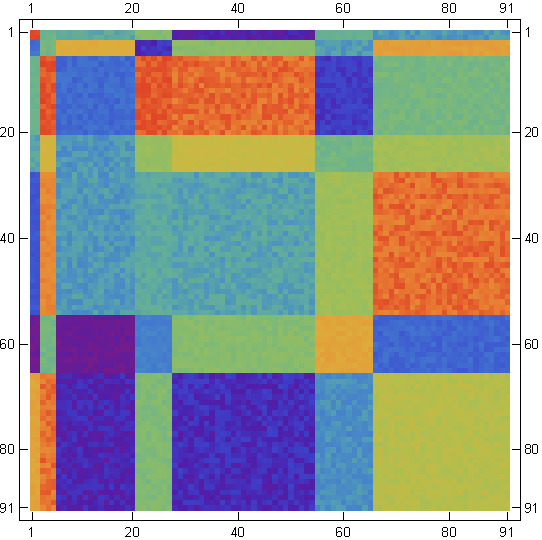
\includegraphics[width=0.8\textwidth]{blockStruct.pdf}
\end{center}
\caption{The block structure for $\forb^2$}
\label{JJ blocks} 
\end{figure}

In \qlanth these blocks are put together by the function \codetext{JJBlockMatrix} which adds together the contributions from the different terms in the Hamiltonian.

\lstinputlisting[language=Mathematica]{./fundefs/JJBlockMatrix.tex}

Once these blocks have been calculated and saved to disk (in the folder \codetext{./hams/}) the function \codetext{HamMatrixAssembly} takes them, assembles the arrays in block form, and finally flattens it to provide a rank-2 array. This are the arrays that are finally diagonalized to find energies and eigenstates.

\lstinputlisting[language=Mathematica]{./fundefs/HamMatrixAssembly.tex}

\section{The effective Hamiltonian} 

Electrons in a multi-electron ion are subject to a number of interactions. They are attracted to the nucleus around which they orbit. Being bundled together with other electrons, they experience repulsion from all of them. Possesing spin, they are also subject to various magnetic interactions. The spin of each electron interacts with the magnetic field generated by either its own orbital angular momentum or that of another electron. And between pairs of electrons, the spin of one can influence the other through the interaction of their respective magnetic dipoles.

To describe the effect of the charges in the lattice surrounding the lattice, the crystal field is introduced. In the simplest of embodiments, the crystal field is simply seen as the electrostatic field due to the surrounding charges. This model, however, has some limitations, but it gives way to a much broader validity based solely on symmetry arguments.

This framework sufficiently describes the interactions within a free ion. However, to extend this model to ions within a crystal, one incorporates this through what is called the crystal field. This is often achieved by considering the electric field that an ion experiences from the surrounding charges in the crystal lattice, a concept referred to as the crystal field effect.

The Hilbert space of a multi-electron ion is a vast stage. In principle the Hilbert space should have a countable infinity of discrete states and an uncountable infinity of states to describe the unbound states. This is clearly too much to handle, but thankfully, this large stage can be put in some order thanks to the exclusion principle. The exclusion principle (together with that graceful tendency of things to drift downwards the energetic wells) provides the shell structure. This shell structure, in turn, makes it possible that an atom with many electrons, can be described effectively as an aggregate of an inert core, and a fewer active valence electrons.  

Take for instance a triply ionized neodymium atom. In principle, this gives us the daunting task of dealing with 57 electrons. However, 54 of them arrange themselves in a xenon core, so that we are only left to deal with only three. Three are still a challenging task, but much less so than fifty seven. Furthermore, the exclusion principle also guides us in what type of orbital we could possibly place these three electrons, in the case of the lanthanide ions, this being the 4f orbitals. But not really, there are many more unoccupied orbitals outside of the xenon core, two of these electrons, if they are willing to pay the energetic price, they could find themselves in a 5d or a 6s orbital.  

Here we shall assume a single-configuration description. Meaning that all the valence electrons in the ions that we study here will all be considered to be located in f-orbitals, or what is the same, that they are described by \fn wavefunctions. This is, however, a harsh approximation, but thankfully one can make some amends to it. The effects that arise in the single configuration description because of omitting all the other possible orbitals where the electrons might find themselves, this is what is called \confint.  

These effects can be brought within the simplified description only through the help of perturbation theory. The task not the usual one of correcting for the energies/eigenvectors given an added perturbation, but rather to consider the effects of using a truncated Hilbert space due to a known interaction. For a detailed analysis of this see Rudzikas' \cite{rudzikas_theoretical_2007} book on theoretical atomic spectroscopy or this article \cite{lindgren_rayleigh-schrodinger_1974} by Lindgren. What results from this are operators that now act solely within the single configuration but with a convoluted coefficient that depends on overlap integrals between different configurations. It is from \confint that the parameters $\casimirAlpha, \casimirBeta, \casimirGamma, \Pk{k}, \Tk{k}$ enter into the description.

The coefficients that result in the Hamiltonian one could try to evaluate, however within the \textbf{semi-empirical} approach these parameters are left to be fitted against experimental data, and perhaps approximated through Hartree-Fock analysis. This approach is only \textit{semi} empirical in the sense that the model parameters are fitted from experimental data, but the model Hamilonian that is fitted is based on a clear physical picture inherited from atomic physics.

Putting all of this together leads to the following Hamiltonian. In there, ``v-electrons'' is shorthand for valence electrons.

\begin{mdframed}
\begin{align} 
	\ham &= \underbracket{\hamKineticSymbol}_{\text{kinetic}}
		 + \underbracket{\hamNuclearCoulombSymbol}_{\text{e:shielded nuc}}
		 + \underbracket{\hamCoulombEESymbol}_{\text{e:e}}
		 + \underbracket{\hamSpinOrbitSymbol}_{\text{spin-orbit}}
		 + \underbracket{\hamSpinSpinSymbol}_{
		 			\substack{
		 				\text{spin:spin} \\ 
		 				\text{and spin:other-orbit}
		 				}
		 			} 
         + \underbracket{\hamSOOplusECSOSymbol}_{
            \substack{
                \text{spin:other-orbit} \\ 
                \text{ec-correlated-spin:orbit}
                }
         } + \\
         & \underbracket{\hamTreesSymbol}_\text{Trees effective op} 
		 + \underbracket{\hamGTwoSymbol}_\text{G${}_2$ effective op} 
		 + \underbracket{\hamSOSevenSymbol}_\text{$\SO{7}$ effective op} 
		 + \underbracket{\ham_{\trispoke}}_{\substack{
            \text{effective} \\
            \text{three-body}}}
         + \underbracket{\hamCrystalFieldSymbol}_{\text{crystal field}} 
         + \underbracket{\hamZeemanSymbol}_{\text{Zeeman}} \\
	\hamKineticSymbol &= -\frac{\hbar^2}{2m_e}\sum_{i=1}^\numE \nabla_i^2 \text{ (kinetic energy of $\numE$ v-electrons)}\\
	\hamNuclearCoulombSymbol &= \hamNuclearCoulomb \text{ (interaction of v-electrons with shielded nuclear charge)} \\
	\ham_\text{e:e} &= \hamCoulombEE \text{ (v-electron:v-electron repulsion)} \\  
	\hamSpinOrbitSymbol &= \begin{cases} 
			\hamSpinOrbit \text{ with } \xi{(r_i)} = \frac{\hbar^2}{2 m^2 c^2 r_i} \frac{\diff{V_\text{sn}(r_i)}}{\diff{r_i}} \\
			\sum_{i=1}^\numE \spinZeta \paren{\op{\sspin}_i \cdot \op{\lorb}_i} {{\substack{
						\text{ with $\spinZeta$ the radial average of $\xi(r_i)$} \\ 
						\text{ or used as phenomenological parameter}  
						}
					}}    
			\end{cases} \\    
	\hamSpinSpinSymbol &= \hamSpinSpin \\  
	\hamSOOplusECSOSymbol &= \hamSOOplusECSO \\ 
	\nonumber \casimir{\anyGroup} &\DEF \text{The Casimir operator of group $\anyGroup$.}\\ 
	\hamTreesSymbol &= \casimirAlpha\casimir{\SO{3}} = \casimirAlpha \op{L}^2 \text{ (Trees effective operator)} \\
	\hamGTwoSymbol      &= \casimirBeta\casimir{\Gtwo} \\
	\hamSOSevenSymbol   &= \casimirGamma\casimir{\SO{7}} \\
	\ham_{\trispoke} &= {\opcolor{T'^{(2)}}}t'_2 + \hamEffectiveThreeBody \text{ (effective 3-body operators $\op{t}_k$)} \\
	\hamCrystalFieldSymbol &= \hamCrystalField {   
		\substack{
			\text{ (crystal field interaction of v-electrons with} \\
			\text{electrostatic field due to surroundings)}
			} 
			}\\
    \hamZeemanSymbol &= -\vec{B} \cdot \op{\mu} = \hamZeeman \text{(interaction with a magnetic field)}
\label{The very effective Hamiltonian}
\end{align}  
\end{mdframed}

It is of some importance to note that the eigenstates that we'll end up with have shoved under the rug all the radial dependence of the wavefunctions. This dependence has been already integrated in the parameters that the Hamiltonian has. 

\subsection{$\hamKineticSymbol$: kinetic energy}

    \begin{equation}
        \hamKineticSymbol = -\frac{\hbar^2}{2m}\sum_{i=1}^N \nabla_i^2 \text{ (kinetic energy of N v-electrons)}
    \end{equation}

    Since our description is limited to a single configuration, the kinetic energy simply contributes a constant energy shift, and since all we care about are energy differences, then this term can be omitted from the analysis.
    
    To interpret the range of energies that result from diagonalizing the Hamiltonian, tt might be instructive, however, to note that this term imparts an energy of about $10\,\eV = 10^6 \Kayser$ to each electron

\subsection{$\hamNuclearCoulombSymbol$: the central field potential}

	In principle the sum over the Coulomb potential should extend over the nuclear charge and over all the electrons in the atom (not just the valence electrons). However, given the shell structure of the atom, the lanthanide ions ``see'' the nuclear charge as shielded by a xenon core. Since every closed shell is a singlet, having spherical symmetry, these shields are literally like spherical shells surrounding the nucleus.
    \begin{equation}
    \hamNuclearCoulombSymbol = -e^2 \sum_{i=1}^{Z} \frac{1}{r_{i}} + e^2 \underbracket{\sum_{i=1}^{\numE}\sum_{j=1}^{Z-\numE} \frac{1}{r_{ij}}}_{\substack{
            \text{Repulsion be-} \\
            \text{tween valence} \\
            \text{and inner shell} \\
            \text{electrons} 
            }
          } \approx \sum_{i=1}^\numE V_\text{sn}(r_i) \text{ (with Z = atomic No.)}
    \end{equation}
	The precise form of $V_\text{sn}(r_i)$ is not of our concern here, all that matters is that we assume that it is spherically symmetric so that we can justify the separation of radial and angular parts of the wavefunctions.

\subsection{$\hamCoulombEESymbol$: e:e repulsion}
 
    \begin{equation}
        \hamCoulombEESymbol = \hamCoulombEE = \sum_{k=0,1,2,3} \Ek \hat{e}^k 
    \end{equation}  

    This term is the first we will not discard. Calculating this term for the \fn configurations was one of the contribution from Slater, as such the parameters we use to write it up are called \textit{Slater integrals}. After the analysis from Slater, Giulio Racah contributed further to the analysis of this term. The insight that Racah had was that if in a given operator one identified the parts in it that transformed nicely according to the different symmetry groups present in the problem, then calculating the necessary matrix element in all \fn configurations can   be greatly simplified.

    The functions used in \ql to compute these LS-reduced matrix elements are \codetext{Electrostatic} and \codetext{fsubk}. In addition to these, the LS-reduced matrix elements of the tensor operators $\op{C}^{(k)}$ and $\op{U}^{(k)}$ are also needed. These functions are based in equations 12.16 and 12.17 from \cite{cowan_theory_1981} as specialized for the case of electrons belonging to a single \fn configuration. By default this term is computed in terms of $\Fk$ Slater integrals, but it can also be computed in of the $\Ek$ Racah parameters, the functions \codetext{EtoF} and \codetext{FtoE} instrumental for going from one representation to the other.
    
    \begin{equation}
    \redbraopket{\forb^n\alpha\LSterm{2S+1}{L}}
        {\hamCoulombEESymbol}
        {\forb^n\alpha'\LSterm{2S'+1}{L'}} = \sum_{k=0,2,4,6} \Fk f_k(n,\alpha{LS},\alpha'{L'S'})
    \end{equation} 
    where
    \begin{multline}
        f_k(n,\alpha{LS},\alpha'{L'S'}) = \frac{1}{2} 
            \kronecker{S}{S'}
            \kronecker{L}{L'}
            \redbraopket{\forb}
                {\op{\mathcal{C}}^{(k)}}
                {\forb}^2 \times \\
            \left\{ 
                \frac{1}{\tpo{L}} \sum_{\alpha''L''} 
                    \redbraopket{\forb^\numE \alpha'' L'' S}
                        {\op{U}^{(k)}}
                        {\forb^\numE \alpha L S} 
                \redbraopket{\forb^\numE \alpha'' L'' S}
                    {\op{U}^{(k)}} 
                    {\forb^\numE \alpha' L S}
                - \kronecker{\alpha}{\alpha'}
                    \frac{\numE \left(4 \forb + 2 - \numE\right)}
                        {(\tpo{\forb})(4 \forb + 1)} 
            \right\}
    \end{multline}       

	\foreach \name in {Electrostatic, fsubk, EtoF, FtoE}{ 
	        \lstinputlisting[language=Mathematica]{./fundefs/\name.tex}
	    }

\subsection{$\hamSpinOrbitSymbol$: spin-orbit}

	The spin-orbit interaction arises from the interaction of the magnetic moment of the electron and the magnetic field that its orbital motion generates. In terms of the central potential $V_{\text{s:n}}$ the spin-orbit term for a single electron is
    \begin{equation}
        \hat{\mathcal{h}}_{\text{s:o}} = \frac{\hbar^2}{2\me^2 c^2} \left(\frac{1}{r}\frac{\mathrm{d}V_{\text{s:n}}}{\mathrm{d}r}\right)\op{l}\cdot{\op{s}} \DEF \zeta{(r)} \op{l}\cdot\op{s}.
    \end{equation}
    Adding this term for all the $\numE$ valence electrons, and replacing $\zeta(r)$ by it's radial average $\spinZeta$ then gives
    \begin{equation}
    \hamSpinOrbitSymbol = \sum_i^{\numE} \spinZeta \dotp{\op{l}_i}{\op{s}_i}.
    \end{equation}

    From equations 2-106 to 2-109 in Wybourne \cite{wybourne_electrostatic_1963} the matrix elements we need are given by
    \begin{multline} 
        \braopket{\alpha LSJ \Msub{J} }{\hamSpinOrbitSymbol}{\alpha' L'S'J'\Msub{J'}} = 
        \spinZeta
        \kronecker{J}{J'}
        \kronecker{\Msub{J}}{\Msub{J'}}
        \braopket{\alpha LSJ \Msub{J} }{\sum_i^{\numE} \dotp{\op{l}_i}{\op{s}_i}}{\alpha' L'S'J\Msub{J}} \\ 
        = \spinZeta \kronecker{J}{J'}
        \kronecker{\Msub{J}}{\Msub{J'}} \phaser{J+L+S'} 
            \sixj{L}{L'}{1}{S'}{S}{J} 
            \braopket{\alpha LS}{\sum_i^{\numE} \dotp{\op{l}_i}{\op{s}_i}}{\alpha' L'S'} \\
        = \spinZeta \kronecker{J}{J'}
        \kronecker{\Msub{J}}{\Msub{J'}} \phaser{J+L+S'} 
            \sixj{L}{L'}{1}{S'}{S}{J} 
            \sqrt{\lorb (\lorb + 1)(2\lorb + 1)} 
            \redbraopket{\alpha{LS}}{\op{V}^{(11)}}{\alpha'L'S'}.
    \end{multline}

    Where $\hat{V}^{(11)}$ is a double tensor operator of rank one over spin and orbital parts defined as 
    \begin{equation}
        \op{V}^{(11)} = \sum_{i=1}^\numE \left( \op{s}\op{u}^{(1)} \right)_i,
    \end{equation}
    where the rank on the spin operator $\op{s}$ has been omitted, and the rank of the orbital tensor operator explicitly as 1.

    In \qlanth the reduced matrix elements for this double tensor operator are calculated by \codetext{ReducedV1k} and aggregated in a static association called \codetext{ReducedV1kTable}. The reduced matrix elements of this operator are calculated using equation 2-101 from Wybourne \cite{wybourne_spectroscopic_1965}:
    \begin{multline} 
        \redbraopket{\lorb^\numE \psi}{\op{V}^{(1k)}}{\lorb^\numE \psi'} = 
            \redbraopket{\lorb^\numE \alpha L S}
                {\op{V}^{(1k)}}
                {\lorb^\numE \alpha'L'S'} =
            \numE 
                \sqrt{\sspin (\sspin + 1) (2\sspin + 1)}
                \sqrt{\tpobraket{S}\tpobraket{L}\tpobraket{S'}\tpobraket{L'}} \times \\
        \sum_{\bar{\psi}}
            \phaser{\bar{S} + \bar{L} + S + L + \lorb + \sspin + k + 1}
            \cfpinv{\psi}{\bar{\psi}}
            \cfp{\bar{\psi}}{\psi'}
            \sixj{S}     {S'}     {1}
                {\sspin} {\sspin} {\bar{S}}
            \sixj{L}     {L'}    {k}
                {\lorb} {\lorb} {\bar{L}}
    \label{eqn:reducedV1k}
    \end{multline}

    In this expression the sum over $\bar{\psi}$ depends on $(\psi,\psi')$ and is over all the states in $\lorb^{n-1}$ which are common parents to both $\psi$ and $\psi'$. Also note that in the equation above, since our concern are f-electron configurations, we have $\lorb = 3$ and $\sspin = \frac{1}{2}$ as is due to the electron.

\foreach \name in {ReducedV1k}{ 
        \lstinputlisting[language=Mathematica]{./fundefs/\name.tex}
    }
 
	These reduced matrix elements are then used by the function \codetext{SpinOrbit}.

\foreach \name in {SpinOrbit}{ 
        \lstinputlisting[language=Mathematica]{./fundefs/\name.tex}
    } 
 
\subsection{$\hamTreesSymbol, \hamGTwoSymbol, \hamSOSevenSymbol$: electrostatic configuration interaction}

    This is a first term where we take into account the contributions from \confint. Rajnak and Wybourne \cite{rajnak_configuration_1963} showed that \confint of the electrostatic interactions corresponding to two-electron excitations from $\forb^\numE$  can be represented through the Casimir operators of the groups $\SO{3}$, $\Gtwo$, and $\SO{7}$. This borrowed from an earlier insight of Trees\cite{trees_l_1952}, who realized that an addition of a term proportional to $L(L+1)$ improved the energy calculations for the second spectrum of manganese (MII) and the third spectrum of iron (FeIII).

    One of these Casimir operators is the familiar $\op{L}^2$ from $\SO{3}$. In analogy to $\op{L}^2$ in which the quantum number $L$ can be used to determine the eigenvalues, in the cases of $\hamGTwoSymbol$ the necessary state label is the $U$ label of the $LS$ term, and in the case of $\hamSOSevenSymbol$ the necessary label is $W$. If $\Lambda_{\Gtwo}\!(U)$ is used to note the eigenvalue of the Casimir operator of $\Gtwo$ corresponding to label $U$, and $\Lambda_{\SO{7}}\!(W)$ the eigenvalue corresponding to state label $W$, then the matrix elements of $\hamTreesSymbol$, $\hamGTwoSymbol$ and $\hamSOSevenSymbol$ are diagonal in all quantum numbers and are given by
    \begin{align}
        \braopket{\lorb^\numE \alpha S L J \Msub{J}}
            {\hamTreesSymbol}
            {\lorb^\numE \alpha' S' L' J' \Msub{J}'} &=
            \casimirAlpha
            \kronecker{\alpha{SLJ}\Msub{J}}{\alpha'{S'L'J'}\Msub{J}'}
            L(L+1) \\
        \braopket{\lorb^\numE U \alpha S L J \Msub{J}}
            {\hamGTwoSymbol}
            {\lorb^\numE U \alpha' S' L' J' \Msub{J}'} &=
            \casimirBeta
            \kronecker{\alpha{SLJ}\Msub{J}}{\alpha'{S'L'J'}\Msub{J}'}
            \Lambda_{\Gtwo}\!(U) \\
        \braopket{\lorb^\numE W \alpha S L J \Msub{J}}
            {\hamSOSevenSymbol}
            {\lorb^\numE W \alpha' S' L' J' \Msub{J}} &=
            \casimirGamma
            \kronecker{\alpha{SLJ}\Msub{J}}{\alpha'{S'L'J'}\Msub{J}'}
            \Lambda_{\SO{7}}\!(W)
    \end{align}

    In \qlanth the role of $\Lambda_{\SO{7}}\!(W)$ is played by the function \codetext{GSO7W}, the role of $\Lambda_{\Gtwo}\!(U)$ by \codetext{GG2U}, and the role of  $\Lambda_{\SO{3}}\!(L)$ by \codetext{CasimirSO3}. These are used by \codetext{CasimirG2}, \codetext{CasimirSO3}, and \codetext{CasimirSO7} which find the corresponding ${U,W,L}$ labels to the LS terms provided to them. Finally, the function \codetext{ElectrostaticConfigInteraction} puts them together.

    \foreach \name in {ElectrostaticConfigInteraction}{
        \lstinputlisting[language=Mathematica]{./fundefs/\name.tex}
    }

\subsection{$\hamSpinSpinSpinOtherOrbitSymbol$: \spinspin and \soo}

    The calculation of the $\hamSpinSpinSpinOtherOrbitSymbol$ is qualitatively different from the previous ones. The previous ones were self-contained in the sense that the reduced matrix elements that we require we also computed on our own. In the case of the interactions that follow from here, we use values from literature for reduced matrix elements either in $\forb^2$ or in $\forb^3$ and then we ``pull'' them up for all $\forb^{\numE}$ configuration with the help of formulas involving \cfps.

    The analysis of \soo, and the \spinspin contributions used in  \qlanth is that of Judd, Crosswhite, and Crosswhite \cite{judd_intra-atomic_1968}. Much as the spin-orbit effect can be extracted as a relativistic correction with the Dirac equation as the starting point. The multi-electron spin-orbit effects can be derived from the Breit operator \cite{bethe_quantum_1957} which is added to the relativistic description of a many-particle system in order to account for retardation of the electromagnetic field
    \begin{equation}
    \ham_B = -\frac{1}{2}e^2 \sum_{i>j} \left[ \left(\alpha_i\cdot\alpha_j\right)\frac{1}{r_{ij}} + \left(\alpha_i\cdot{\vec{r}_{ij}}\right)\left(\alpha_j\cdot\vec{r}_{ij}\right) \frac{1}{r_{ij}^3} \right].
    \end{equation}

    When this operator is expanded in powers of $v/c$, a number of non-relativistic inter-electron interactions result. Two of them being the \soo and \spinspin interactions.

    As usual, the radial part of the Hamiltonian is averaged, which in this case gives appearance to the Marvin integrals
    \begin{equation} 
    \Mk{k} \DEF \frac{e^2\hbar^2}{8m^2c^2} \braopket{(nl)^2}{\frac{r_<^k}{r_>^{k+3}}}{(nl)^2}
    \end{equation}

    With these, the expression for the \spinspin term is \cite{judd_intra-atomic_1968}
    \begin{multline}
    \ham_{s:s} = -2 \sum_{i\neq{j}}
        \sum_k \Mk{k}
            \sqrt{(k+1)(k+2)(2k+3)} 
            \redbraopket{\lorb}{\Ck{k}}{\lorb} 
            \redbraopket{\lorb}{\Ck{k+2}}{\lorb}
            \left\{
                \wdouble{i}{1}{k}
                \wdouble{j}{1}{k+2}
            \right\}^{(2,2)0}
    \end{multline}
    and the one for \soo 
    \begin{multline}
        \ham_{s:oo} = \sum_{i\neq{j}} 
            \sum_k 
                \sqrt{(k+1)(2\lorb+k+2)(2\lorb-k)}  \times \\ 
        \left[ \left\{ \wdouble{i}{0}{k+1} \wdouble{j}{1}{k} \right\}^{(11)0} 
        \left\{ \Mk{k-1}
            \redbraopket{\lorb}
                {\Ck{k+1}}
                {\lorb}^2
            +
            2 \Mk{k} \redbraopket{\lorb}{\Ck{k}}{\lorb}^2
        \right\} + \right. \\
        \left.
            \left\{ \wdouble{i}{0}{k}\wdouble{j}{1}{k+1} \right\}^{(11)0} 
                \left\{ \Mk{k} 
                    \redbraopket{\lorb}{\Ck{k}}{\lorb}^2
                    + 2 \Mk{k-1}
                    \redbraopket{\lorb}{\Ck{k+1}}{\lorb}^2
                \right\}
        \right].
    \end{multline} 

    In the expressions above $\wdouble{i}{\kappa}{k}$ is a double tensor operator of rank $\kappa$ over spin, of rank $k$ over orbit, and acting on electron $i$. It is defined by its reduced matrix elements as
    \begin{equation} 
    \redbraopket{\lorb}
        {\wdouble{}{\kappa}{k}}
        {\lorb}
        = \sqrt{\tpobraket{\kappa}
            \tpobraket{k}
        }
    \end{equation} 

    The complexity of the above expressions for can be identified by identifying them with the scalar part of two new double tensors $\Txyz{1}{1}{0}$ and $\Txyz{2}{2}{0}$ such that
    \begin{align}
    \sqrt{5}\Txyz{2}{2}{0} &\DEF \hamSpinSpinSymbol \\
    -\sqrt{3}\Txyz{1}{1}{0} &\DEF \hamSpinOtherOrbitSymbol.
    \end{align}

    In terms of which the reduced matrix elements in the $\LSJbasis$ basis can be obtained by
    \begin{equation}
        \braopket{\gamma{SLJ}}{\ham}{\gamma'{S'L'J'}} = \kronecker{J}{J'} \sixj{S'}{L'}{J}{L}{S}{t} \redbraopket{\gamma{SL}}{\Txyz{t}{t}{}}{\gamma'{S'L'}}.
    \label{SLtoSLJ for Ttt}
    \end{equation}

    This above relationship is used in \qlanth in the functions \codetext{SpinSpin} and \codetext{SOOandECSO}.

    \foreach \name in {SpinSpin, SOOandECSO}{
        \lstinputlisting[language=Mathematica]{./fundefs/\name.tex}
    }

    For two-electron operators such as these, the matrix elements in $\forb^\numE$ are related to those in $\forb^{\numE-1}$ through equation 4 in Judd et al \cite{judd_intra-atomic_1968}
    \begin{multline}
        \redbraopket{\forb^\numE\psi}
        	{\Txyz{t}{t}{}}
        	{\forb^\numE\psi'} 
        = \frac{\numE}{\numE-2} 
        \sum_{\bar{\psi},\bar{\psi}'}
        \phaser{\bar{S}+\bar{L}+\sspin+\lorb+S'+L'}
        \sqrt{\tpobraket{S}\tpobraket{S'}\tpobraket{L}\tpobraket{L'}} \times \\
        \cfpinv{\psi}{\bar{\psi}}
        \cfpinv{\psi'}{\bar{\psi}'} 
        \sixj{S}{t}{S'}{\bar{S}'}{\sspin}{\bar{S}}
        \sixj{L}{t}{L'}{\bar{L}'}{\lorb}{\bar{L}}
        \redbraopket{\forb^{\numE-1}\bar{\psi}}
        {\Txyz{t}{t}{}}{\forb^{\numE-1}]\bar{\psi}'}.
    \label{double cfp escalator}
    \end{multline}
    Where the sum runs over the terms $\bar{\psi}$ and $\bar{\psi}'$ in $\forb^{\numE-1}$ which are parents common to $\psi$ and $\psi'$. Using these the matrix elements of $\Txyz{1}{1}{}$ and $\Txyz{2}{2}{}$ in $\forb^2$ can be used to compute all the reduced matrix elements in  $\forb^\numE$. These could then be used, together with \eqnref{SLtoSLJ for Ttt} to obtain the matrix elements of $\hamSpinSpinSymbol$ and $\hamSpinOtherOrbitSymbol$. This is done for $\hamSpinSpinSymbol$, but not for $\hamSpinOtherOrbitSymbol$, since this term is traditionally computed (with a slight modification) at the same as the electrostically-correlated-spin-orbit (see next section).

    These equations are implemented in \qlanth through the following functions: \codetext{Generate{\-}T22{\-}Table}, \codetext{ReducedT22infn}, \codetext{ReducedT22inf2}, \codetext{ReducedT11inf2}. Where \codetext{ReducedT22inf2} and \codetext{ReducedT11inf2} provide the reduced matrix elements for $\Txyz{1}{1}{}$ and $\Txyz{2}{2}{}$ in $\forb^2$ as provided in table II of \cite{judd_intra-atomic_1968}.

    \foreach \name in {GenerateT22Table, ReducedT22infn, ReducedT22inf2, ReducedT11inf2}{
        \lstinputlisting[language=Mathematica]{./fundefs/\name.tex}
    }

\subsection{$\hamECSOSymbol$: \ecso}

    In the same paper \cite{judd_intra-atomic_1968} that describes the \spinspin and \soo interactions, consideration is also given to the emergence of additional corrections due to configuration interaction as described by the following operator (which is what results from the application of perturbation theory to \textit{second} order) (page.  134 of \cite{judd_intra-atomic_1968})
    \begin{equation}
        \ham_{\text{ci}} = -\sum_\chi \sum_i \frac{1}{E_\chi}\xi(r_i) 
            \left(  
                \op{\sspin}_i\cdot\op{\lorb}_i
            \right) \ket{\chi} \bra{\chi} \CoulombNonCentral
            - \frac{1}{E_\chi}\CoulombNonCentral \ket{\chi}\bra{\chi} \xi(r_i) 
                \left( 
                    \op{\sspin}_i\cdot\op{\lorb}_i
                \right) 
    \end{equation} 
    where $\xi(r_h) (\op{\sspin}_h\cdot\op{\lorb}_h)$ is the customary spin-orbit interaction, $E_\chi$ is the energy of state $\ket{\chi}$, $i$ is a label for the valence electrons, $\CoulombNonCentral$ stands for the Coulomb interaction, and $\ket{\chi}$ are states in the configurations to which one is ``interacting'' with. Since this term includes both the electrostatic term and the spin-orbit one, this is called the \ecso interaction.

    This operator can be identified with the scalar component of a double tensor operator of rank 1 both for the spin and orbital parts of the wavefunction. 
    \begin{equation}
        \ham_{\text{ci}} = - \sqrt{3}\,\txyz{1}{1}{0}
    \end{equation}

    Judd \textit{et al.} then go on to list the reduced matrix elements of this operator in the $\forb^2$ configuration. When this is done the Marvin integrals $\Mk{k}$ appear again, but a second set of parameters, the \textit{pseudo-magnetic} parameters $\Pk{k}$, is also necessary
    \begin{equation}
        \Pk{k} = 6 \sum_{f'}
            \frac{\zeta_{ff'}}
                {E_{ff'}}
                R^{(k)}(ff,ff') \text{ for }k=0,2,4,6.
    \end{equation}
    Where $f$ notes the radial eigenfunction attached to an f-electron wavefunction, and $f'$ similarly but for a configuration different from $\forb^\numE$. And where
    \begin{align}
        \zeta_{ff'} &\DEF \braopket{f}{\xi(r)}{f'} \\
        R^{(k)}(ff,ff') &\DEF e^2 \braopket{f_1f_2}{\frac{r_<^k}{r_>^{k+1}}}{f_1f_2'}.
    \end{align}

    In the semi-empirical approach embodied by $\qlanth$, calculating these quantities \textit{ab-initio} is not the objective, rendering the precise definition of these parameters non-essential. Nonetheless, these expressions frequently serve to justify the ratios between different orders of these quantities. Consequently, both the set of three $\Mk{k}$ and the set of $\Pk{k}$ ultimately rely on a single free parameter each. Such parsimony is desirable given the large number of parameters (about 20) that the Hamiltonian ends up having.

    Judd \textit{et al.} further note that $\Pk{0}$ is proportional to the spin orbit operator, and as such its effect is absorbed by the standard spin-orbit parameter $\spinZeta$. They also developed an alternative approach based on group theory arguments. They put together the \soo and the \ecso as a sum of operators $\op{z}_i$ with useful transformation rules 
    \begin{equation}
        \redbraopket{\psi}{\Txyz{1}{1}{} + \txyz{1}{1}{}}{\psi'} = \sum a_i \redbraopket{\psi}{\hat{z}_i}{\psi'}.
    \end{equation}

    At this stage a subtle point needs to be raised. As Judd points out, in the sum above, the term $\op{z}_{13}$ that contributes with a tensorial character equal to that of the regular spin-orbit operator. As such, if the goal is obtaining a parametric Hamiltonian that can be fit with uncorrelated parameters, it is then necessary to subtract this part from $\Txyz{1}{1}{} + \txyz{1}{1}{}$. This point was clarified by Chen \textit{et al.} \cite{chen_few_2008}. Because of this the final form of the operator contributing both to \soo and the \ecso is
    \begin{equation}
        \hamSpinOtherOrbitSymbol + \hamECSOSymbol = \Txyz{1}{1}{} + \txyz{1}{1}{} - \frac{1}{6}a_{13}\op{z}_{13}
        \label{SOO ECSO sum}
    \end{equation}
    where
    \begin{equation}
        a_{13} = -33 \Mk{0} + 3 \Mk{2} + \frac{15}{11} \Mk{4} - 6 \Pk{0} + \frac{3}{2} \left(\frac{35}{225} \Pk{2} + \frac{77}{1089} \Pk{4} + \frac{25}{1287} \Pk{6}\right).
    \end{equation}

    In \qlanth the contributions from \spinspin, \soo, and \ecso are put together by the function \codetext{MagneticInteractions}. That function queries precomputed values from two associations \codetext{SpinSpinTable} and \codetext{SOOandECSOTable}. In turn these two associations are generated by the functions \codetext{GenerateSpinOrbitTable} and \codetext{GenerateSOOandECSOTable}. Note that both \spinspin and \soo end up contributing through $\Mk{k}$, however there doesn't seem to be consensus about adding them together, as such \qlanth allows including or excluding the \spinspin contribution, this is done with a control parameter $\sigma_{SS}$ (1 for including, 0 for excluding).

    \foreach \name in {MagneticInteractions, GenerateSpinOrbitTable, GenerateSOOandECSOTable}{
        \lstinputlisting[language=Mathematica]{./fundefs/\name.tex}
    }

    The function \codetext{GenerateSpinSpinTable} calls the function \codetext{SpinSpin} over all possible combinations of the arguments $\{\numE, SL, S'L', J\}$. In turn the function \codetext{SpinSpin} queries the precomputed values of the the double tensor $\Txyz{2}{2}{}$ which are stored in the association \codetext{T22Table}. 


    \foreach \name in {GenerateSpinSpinTable, SpinSpin}{ 
        \lstinputlisting[language=Mathematica]{./fundefs/\name.tex}
    }

    The association \codetext{T22Table} is computed by the function \codetext{GenerateT22Table}. This function populates \codetext{T22Table} with keys of the form $\{\numE, SL, S'L'\}$. It does this by using the function \codetext{ReducedT22inf2} in the base case of $\forb^2$, and \codetext{ReducedT22infn} for configurations above $\forb^2$. When \codetext{ReducedT22infn} is called the sum in \eqnref{double cfp escalator} is carried out using $t=2$. When \codetext{ReducedT22inf2} is called the reduced matrix elements from \cite{judd_intra-atomic_1968} are used. 

    \foreach \name in {GenerateT22Table, ReducedT22infn, ReducedT22inf2}{
        \lstinputlisting[language=Mathematica]{./fundefs/\name.tex}
    }

    The function \codetext{GenerateSOOandECSOTable} calls the function \codetext{SOOandECSO} over all possible combinations of the arguments $\{\numE, SL, S'L', J\}$ and uses their values to populate the association \codetext{SOOandECSOTable}. In turn the function \codetext{SOOandECSO} queries the precomputed values of \eqnref{SOO ECSO sum} as stored in the association \codetext{SOOandECSOLSTable}. 

    \foreach \name in {GenerateSOOandECSOTable, SOOandECSO, SOOandECSO}{
        \lstinputlisting[language=Mathematica]{./fundefs/\name.tex}
    }

    The association \codetext{SOOandECSOLSTable} is computed by the function \codetext{GenerateSOOandECSOLSTable}. This function populates \codetext{SOOandECSOLSTable} with keys of the form $\{\numE, SL, S'L'\}$. It does this by using the function \codetext{ReducedSOOandECSOinf2} in the base case of $\forb^2$, and \codetext{ReducedSOOandECSOinfn} for configurations above $\forb^2$. When \codetext{ReducedSOOandECSOinfn} is called the sum in \eqnref{double cfp escalator} is carried out using $t=1$. When \codetext{ReducedSOOandECSOinf2} is called the reduced matrix elements from \cite{judd_intra-atomic_1968} are used.

    \foreach \name in {ReducedSOOandECSOinfn, ReducedSOOandECSOinf2}{
        \lstinputlisting[language=Mathematica]{./fundefs/\name.tex}
    }

\subsection[$\ham_3$: three-body effective operators]{$\ham_{\trispoke}$: three-body effective operators}


The three-body operators arise in the Hamiltonian due to the configuration interaction effects of the Coulomb repulsion. More specifically, they originate from configuration interaction between the ground configuration $(4\forb)^{\numE}$ and single electron excitations to the $(4\forb)^{\numE\pm{1}}(n'\lorb')^{\mp{1}}$ configurations.

The operators that can be used to span the resulting effects were initially studied by Wybourne and Rajnak in 1963 \cite{rajnak_configuration_1963}, their analysis was complemented soon after by Judd \cite{judd_three-particle_1966}, and revisited again by Judd in 1984 \cite{judd_complete_1984}.

This model interaction is spanned by a set of 14 $\op{t}_i$ of operators ($\op{t}$ fron \textit{t}hree)
\begin{equation}
\ham_{\trispoke} = {\opcolor{T'^{(2)}}}\op{t}'_2 + {\opcolor{T'^{(11)}}}\op{t}'_{11} \hamEffectiveThreeBody, 
\end{equation}
where $\op{t}_2'$ and $\op{t}_{11}'$ are operators that were initially included but which were later replaced by $\op{t}_2$ and $\op{t}_{11}$ (see \cite{judd_complete_1984}). \qlanth includes the legacy operator $\op{t}_2'$ since it was used for important work during and before the 1980s.

The omission of some indices in this sum has to do with the fact that the way in which these are defined in terms of their index (see \cite{judd_three-particle_1966}) gives rise to two-body operators which can be absorbed by the two-body terms in the Hamiltonian. As such, it is not so much that they are not included, but rather that their effects are considered to be accounted for elsewhere. This is representative of a common feature of configuration interaction: it gives rise to new intra-configuration operators, but it also contributes to already present operators; this makes it harder to approximate the model parameters \textit{ab-initio}, but is not a practical obstacle for the semi-empirical approach (although it certainly complicates the physical interpretation that each parameter has).

Furtermore, it is often the case that the operator set is limited to the subset \{2,3,4,6,7,8\}; a practice that is justified \textit{post-facto} after seeing that these are sufficient to describe the data.

The calculation of a three body operator matrix elements across the $\forb^{\numE}$ configurations is analogous to how a two-body operator is calculated. Except that in this case what is needed are the reduced matrix elements in $\forb^3$ and the equation that is used to propagate these across the other configurations is as in equation 4 of \cite{judd_three-particle_1966} (adding the explicit dependence on $J$ and $\Msub{J}$):
\begin{equation} 
	\braopket{\forb^{\numE}\psi}
		{\op{t}_i}
		{\forb^{\numE}\psi'} =
		\kronecker{J}{J'}
		\kronecker{\Msub{J}}{\Msub{J}'} 
		\frac{\numE}{\numE-3} 
		\sum_{\bar{\psi}\bar{\psi}'}
			\cfpinv{\psi}{\bar{\psi}}
        	\cfpinv{\psi'}{\bar{\psi}'}
        	\braopket{\forb^{\numE-1}\bar{\psi}}{\op{t}_i}{\forb^{\numE-1}\bar{\psi}'}.
\label{eqn:three body escalator}
\end{equation}

The sum in this expression runs over the parents in $\forb^{\numE-1}$ that are common to both the daughter terms $\psi$ and $\psi'$ in $\forb^{\numE}$. The equation above yielding LSJMJ matrix elements, and being diagonal in $J$, $\Msub{J}$ as is due to a scalar operator.

In \qlanth this is all implemented in the function \codetext{GenerateThreeBodyTables}. Where the matrix elements in $\forb^3$ are from \cite{judd_complete_1984}, where the data has been digitized in the files \codetext{Judd1984-1.csv} and \codetext{Judd1984-2.csv}, which are parsed through the function \codetext{ParseJudd1984}.
 
 In \codetext{GenerateThreeBodyTables} a special case is made for $\op{t}_2$ and $\op{t}_{11}$ for which primed variants $\op{t}_2'$ and $\op{t}_{11}'$ are calculated differently beyond the half filled shell. In the case of the other operators, beyond $\forb^7$ the matrix elements simply see a global sign flip, whereas in the case of $\op{t}_2'$ and $\op{t}_{11}'$ the \cfps beyond $\forb^7$ are used. This yields the unexpected result that in the $\forb^{12}$ configuration, which corresponds to two holes, there is a non-zero three body operator $\op{t}_2'$. This is an arcane result that was corrected by Judd in 1984 \cite{judd_complete_1984}, but which lingered long enough that important work in the 1980s was calculated with it. When calculations are carried out if $\op{t}_2'$ is used then $\op{t}_2$ should not be used and vice versa.
 
 One additional feature of $\hat{t}_2'$ that needs to be accounted for, is that it doesn't have the simple relationship for conjugate configurations that all the other $\hat{t}_i$ operators have. For the sake of parsimony, and to avoid having to explicitly store matrix elements beyond $\forb^7$ \qlanth takes the approach of adding a control parameter \codetext{t2Switch} which needs to be set to 1 if below or at $\forb^7$ and set to 0 if above $\forb^7$.
 
 \foreach \name in {GenerateThreeBodyTables, ParseJudd1984}{ 
        \lstinputlisting[language=Mathematica]{./fundefs/\name.tex}
    }
 
\subsection{$\hamCrystalFieldSymbol$: crystal-field} 

	The crystal-field partially accounts for the influence of the surrounding lattice on the ion. The simplest picture of this influence imagines the lattice as responsible for an electric field felt at the position of the ion. This electric field corresponding to an electrostatic potential described as a multipolar sum of the form:  
    \begin{equation}   
    V(r_i, \theta_i, \phi_i) = \sum_{k=1}^\infty \sum_{q=-k}^k \Akq r_i^k \Ckq{k}{q}(\theta_i, \phi_i) 
    \end{equation}  

    Where we have chosen a coordinate system with its origin at the position of the nucleus, and in which we only have positive powers of the distance $r_i$ since here we have expanded the contributions from all the surrounding ions as a sum over spherical harmonics centered at the position of the nucleus, without $r$ ever large enough to reach any of the positions of the lattice ions. 

    Furthermore, since we have $\numE$ valence electrons, then the total crystal field potential is 
    \begin{equation}
        \hamCrystalFieldSymbol(\vec{r}) = 
        	\sum_{i=1}^\numE
        	\sum_{k=0}^\infty
        	\sum_{q=-k}^{k} \Akq r_i^k \Ckq{k}{q}(\theta_i,\phi_i).
    \label{eqn:crystal sum}
    \end{equation}

    And if we average the radial coordinate,
    \begin{equation}
        \hamCrystalFieldSymbol = \sum_{i=1}^\numE \sum_{k=1}^\infty \sum_{q=-k}^{k} \Bcomplexkq{k}{q} {\Ckq{k}{q}}\!(i) 
    \end{equation}
    where the radial average is included as
    \begin{equation}
    \Bcomplexkq{k}{q} \DEF \Akq {\langle 4f | r^k | 4f\rangle}.
    \end{equation}
    
    $\Bcomplexkq{k}{q}$ may be complex in general. However, since the sum in \eqnref{eqn:crystal sum} needs to result in a real and Hermitian operator, there are restrictions on $\Bcomplexkq{k}{q}$ that need to be accounted for. Once the behavior of $\Ckq{k}{q}$ under complex conjugation is considered, $\Ckq{k}{q}{}^* = \phaser{q}\Ckq{k}{-q}$, it is necessary that
    \begin{equation}
    	\Bcomplexkq{k}{q} = \phaser{q}\Bcomplexkq{k}{-q}^{*}.
    \end{equation}
    
    Presently the sum over $q$ spans both its negative and positive values. This can be limited to only the non-negative values of $q$. Separating the real and imaginary parts of $\Bcomplexkq{k}{q}$ such that $\Bcomplexkq{k}{q} = \Bkq{k}{q} + i \Skq{k}{q}$ for $q\neq{0}$ and $\Bcomplexkq{k}{0} = 2\Bkq{k}{0}$ the sum for the crystal field can then be written as
    \begin{equation}
        \hamCrystalFieldSymbol(\vec{r}) = 
        	\sum_{i=1}^\numE
        	\sum_{k=0}^\infty
        	\sum_{q=0}^{k} \Bkq{k}{q} \left(\Ckq{k}{q} + \phaser{q}\Ckq{k}{-q}\right) + i \Skq{k}{q} \left(\Ckq{k}{q} - \phaser{q}\Ckq{k}{-q}\right).
    \label{eqn:better crystal sum}
    \end{equation}
    
    A staple of the Wigner-Racah algebra is writing up operators on interest in terms of standard ones for which the matrix elements are straightforward.  One such operator is the unit tensor operator $\hat{u}^{(k)}$ for a single electron. The Wigner-Eckart theorem --on which all of this algebra is an elaboration-- effectively separates the dynamical and geometrical parts of a given interaction; the unit tensor operators isolate the geometric contributions. This irreducible tensor operator $\hat{u}^{(k)}$ is defined as the tensor operator having the following reduced matrix elements (written in terms of the triangular delta, see section on notation):
    \begin{equation}
    \redbraopket{\ell}{\hat{u}^{(k)}}{\ell'} = 1.
    \end{equation}

    In terms of this tensor one may then define the symmetric (in the sense that the resulting operator is equitable among all electrons) unit tensor operator for $\numE$ particles as
    \begin{equation}
        \hat{U}^{(k)} = \sum_{i}^{\numE} \op{u}^{(k)}_i.
    \end{equation}

    This tensor is relevant to the calculation of the above matrix elements since 
    \begin{equation}
        \Ckq{k}{q} = \redbraopket{\lorb}
                    {\Ck{k}}
                    {\lorb{'}} \op{u}^{(k)}_q 
            = \phaser{\lorb}
            \sqrt{\tpobraket{\lorb}\tpobraket{\lorb{'}}}
            \threej{\lorb}{k}{\lorb'}{0}{0}{0} \op{u}^{(k)}_q.
    \end{equation}

    With this the matrix elements of $\hamCrystalFieldSymbol$ in the $\LSJMbasis$ basis are: 
    \begin{align}
        \overbracket{\braopket{\lorb^\numE \alpha SLJ \Msub{J}}{\hamCrystalFieldSymbol}{\lorb^\numE \alpha'S L' J' \Msub{J'}}}^{\text{Wybourne eqn. 6-3}} &= \sum_{k=1}^\infty\sum_{q=-k}^k    
        \Bcomplexkq{k}{q} 
            \braopket{\lorb^\numE \alpha SLJ\Msub{J}}
                {\op{U}^{(k)}_q}
                {\lorb^\numE \alpha'SL'J'\Msub{J'}} 
            \redbraopket{\lorb}
                {\op{C}^{(k)}}
                {\lorb} 
    \label{HCFsum}
    \end{align}

    where the matrix elements of $\op{U}^{(k)}_q$ can be resolved with a 3j symbol as
    \begin{align}
        \overbracket{\braopket{\lorb^\numE \alpha S L J \Msub{J}}
            {\op{U}^{(k)}_q}
            {\lorb^\numE \alpha' S' L' J' \Msub{J'}}}^
            {\text{Wybourne eqn. 6-4}}
            &= 
            \phaser{J-\Msub{J}}
            \threej{J}{k}{J'}
                {-\Msub{J}}{q}{\Msub{J'}}
        \redbraopket{\lorb^\numE \alpha S L J}
                {\op{U}^{(k)}}
                {\lorb^\numE \alpha' S' L'}
    \end{align}
    and reduced a second time with the inclusion of a 6j symbol resulting in
    \begin{align}
        \nonumber \overbracket{\redbraopket{\lorb^\numE \alpha S L J}
            {\op{U}^{(k)}}
            {\lorb^\numE \alpha' S' L'}}^
            {\text{Wybourne eqn. 6-5}}
        &= 
        \phaser{S+L+J'+k} 
        \sqrt{\tpobraket{J}\tpobraket{J'}} \times \\
        & \sixj{J}{J'}{k}{L'}{L}{S}
        \redbraopket{\lorb^\numE \alpha S L}
            {\op{U}^{(k)}}
            {\lorb^\numE \alpha' S' L'}.
    \end{align}

    This last reduced matrix element is finally computed with a sum over $\bar{\alpha}\bar{L}\bar{S}$ which are the parents in configuration $\forb^{\numE-1}$ which are common to $\ket{\alpha L S}$ and $\ket{\alpha' L' S'}$ from configuration $\forb^{\numE}$:
    \begin{multline}
    \overbracket{\redbraopket{\lorb^\numE \alpha S L} 
        {\op{U}^{(k)}}
        {\lorb^\numE \alpha' S' L'}}^{\text{Cowan eqn. 11.53}} = \kronecker{S}{S'} \numE \phaser{\lorb + L + k}
            \sqrt{\tpobraket{L}\tpobraket{L'}} \times \\
    \sum_{\bar{\alpha}\bar{L}\bar{S}} 
        \phaser{\bar{L}} \sixj{\lorb}{k}{\lorb}{L}{\bar{L}}{L'}
        \cfpinv{\lorb^\numE \alpha L S}
            {\lorb^{\numE - 1}\bar{\alpha}\bar{L}\bar{S}}
        \cfp{\lorb^{\numE -1}\bar{\alpha}\bar{L}\bar{S}}{\lorb^\numE\alpha'L'S'}.
    \label{eqn:ReducedUk}
    \end{multline}

    From the $\redbraopket{\lorb}{\op{C}^{(k)}}{\lorb}$, and given that we are using $\lorb = \forb = 3$ we can see that by the triangular condition $\tricondition{3,k,3}$ the non-zero contributions only come from $k=0,1,2,3,4,5,6$. An additional selection rule on $k$ comes from considerations of parity. Since both the bra and the ket in $\braopket{\lorb^\numE \alpha SLJ \Msub{J}}{\hamCrystalFieldSymbol}{\lorb^\numE \alpha'S L' J' \Msub{J'}}$ have the same parity, then the overall parity of the braket is determined by the parity of $\Ckq{k}{q}$, and since the parity of $\Ckq{k}{q}$ is $\phaser{k}$ then for the braket to be non-zero we require that $k$ should also be even. In view of this, in all the above equations for the crystal field the values for $k$ should be limited to $2,4,6$. The value of $k=0$ having been omitted from the start since this only contributes a common energy shift. Putting everything together:
       	\begin{equation}
        \hamCrystalFieldSymbol(\vec{r}) = 
        	\sum_{i=1}^\numE
        	\sum_{k=2,4,6}
        	\sum_{q=0}^{k} \Bkq{k}{q} \left(\Ckq{k}{q} + \phaser{q}\Ckq{k}{-q}\right) + i \Skq{k}{q} \left(\Ckq{k}{q} - \phaser{q}\Ckq{k}{-q}\right).
    	\label{eqn:supreme crystal sum}
    	\end{equation}

    The above equations are implemented in \qlanth by the function \codetext{CrystalField}. This function puts together the symbolic sum in \eqnref{HCFsum} by using the function \codetext{Cqk}. \codetext{Cqk} then uses the diagonal reduced matrix elements of $\Ckq{k}{q}$ and the precomputed values for \codetext{Uk} (stored in \codetext{ReducedUkTable}).

    The required reduced matrix elements of $\hat{U}^{(k)}$ are calculated by the function \codetext{ReducedUk}, which is used by \codetext{GenerateReducedUkTable} to precompute its values.
    
\foreach \name in {Bqk, Sqk, Cqk, CrystalField, ReducedUk}{ 
        \lstinputlisting[language=Mathematica]{./fundefs/\name.tex}
    }


\subsection{$\hat{\mu}$ and $\hamZeemanSymbol$: the magnetic dipole operator and the Zeeman term}

In Hartree atomic units, the operator associated with the magnetic dipole operator for an electron is
\begin{equation}
\hat{\mu} = -\muBohr \left(\op{L} + g_s\op{S} \right)^{(1)}, \text{with }\muBohr=1/2.
\end{equation}
Here we have emphasized the fact that the magnetic dipole operator corresponds to a rank-1 spherical tensor operator.

In the $\LSJMbasis$ basis that we use in \qlanth the LSJ reduced-matrix elements are computed using equation 15.7 in \cite{cowan_theory_1981}
\begin{multline}
    \redbraopket{\alpha{LSJ}}
        {\left(\op{L} + g_s \op{S}\right)^{(1)}}
        {\alpha'{L'S'J'}} =
    \kronecker{\alpha{LSJ}}
        {\alpha'{L'S'J'}}
    \sqrt{J(J+1)(2J+1)} + \\
    \kronecker{\alpha{LS}}
        {\alpha'{L'S'}}
    \phaser{L+S+J+1}
    \sqrt{\tpobraket{J}\tpobraket{J}}
    \sixj{L}{S}{J}{1}{J'}{S}
\end{multline}

And then those reduced matrix elements are used to resolve the $\Msub{J}$ components for $q=-1,0,1$ through Wigner-Eckart  
\begin{multline}
    \braopket{\alpha{LSJ}\Msub{J}}
        {\left(\op{L} + g_s \op{S}\right)^{(1)}_q}
        {\alpha'{L'S'J'}\Msub{J'}} = \\
    \phaser{J-\Msub{J}}
    \threej{J}{1}{J'}{-\Msub{J}}{q}{\Msub{J}'}
    \redbraopket{\alpha{LSJ}}
        {\left(\op{L} + g_s \op{S}\right)^{(1)}}
        {\alpha'{L'S'J'}} 
\end{multline} 
These two above are put together in \codetext{JJBlockMagDip} for given $\{\numE, J, J'\}$ returning a rank-3 array representing the quantities $\{\Msub{J},\Msub{J}',q\}$.

\foreach \name in {JJBlockMagDip}{
    \lstinputlisting[language=Mathematica]{./fundefs/\name.tex}
}

The $JJ'$ blocks that are generated with this function are then put together by \codetext{MagDipoleMatrixAssembly} into the final matrix form and the cartesian components calculated according to 
\begin{align}
	\op{\mu}_x &= \frac{\op{\mu}^{(1)}_{-1} - \op{\mu}^{(1)}_{+1}}{\sqrt{2}} \\
	\op{\mu}_y &= i\frac{\op{\mu}^{(1)}_{-1} + \op{\mu}^{(1)}_{+1}}{\sqrt{2}} \\
	\op{\mu}_z &= \op{\mu}^{(1)}_{0}
\end{align}

\foreach \name in {MagDipoleMatrixAssembly}{
    \lstinputlisting[language=Mathematica]{./fundefs/\name.tex}
}

Using the cartesian components of the magnetic dipole operator, the matrix elements of the Zeeman term can then be evaluated. This term can be included in the Hamiltonian through an option in \codetext{HamMatrixAssembly}. Since the magnetic dipole operator is calculated in atomic units, and it seeming desirable that the input units of the magnetic field be Tesla, a conversion factor is included so that the final terms be congruent with the energy units assumed in the other terms in the Hamiltonian, namely the pseudo-energy unit Kayser ($\text{cm}^{-1}$). The conversion factor is called \codetext{TeslaToKayser} in the file \codetext{qonstants.m}.

\subsection[Going beyond $f^7$]{Going beyond $f^7$}

In most cases all matrix elements in \qlanth are only calculated up to and including $\forb^7$. Beyond $\forb^7$ adequate changes of sign are enforced to take into account the equivalence that can be made between $\forb^{\numE}$ and $\forb^{14-\numE}$ as given by \eqnref{eqn:sign change double tensor op} and \eqnref{eqn:sign change tensor op}. 

\begin{mdframed}
\begin{align} 
	\ham &= \underbracket{\hamKineticSymbol}_{\text{kinetic}}
		 + \underbracket{\hamNuclearCoulombSymbol}_{\text{e:shielded nuc}}
		 + \underbracket{\hamCoulombEESymbol}_{\text{e:e}}
		 + \underbracket{\hamSpinOrbitSymbol}_{\text{spin-orbit}}
		 + \underbracket{\hamSpinSpinSymbol}_{
		 			\substack{
		 				\text{spin:spin} \\ 
		 				\text{and spin:other-orbit}
		 				}
		 			} 
         + \underbracket{\hamSOOplusECSOSymbol}_{
            \substack{
                \text{spin:other-orbit} \\ 
                \text{ec-correlated-spin:orbit}
                }
         } + \\
         & \underbracket{\hamTreesSymbol}_\text{Trees effective op} 
		 + \underbracket{\hamGTwoSymbol}_\text{G${}_2$ effective op} 
		 + \underbracket{\hamSOSevenSymbol}_\text{$\SO{7}$ effective op} 
		 + \underbracket{\ham_{\trispoke}}_{\substack{
            \text{effective} \\
            \text{three-body}}}
         + \underbracket{\hamCrystalFieldSymbol}_{\text{crystal field}} 
         + \underbracket{\hamZeemanSymbol}_{\text{Zeeman}} 
\label{The very effective Hamiltonian}
\end{align}  
\end{mdframed}

This is enforced when the function \codetext{HamMatrixAssembly} is called. In there \codetext{HoleElectronConjugation} is the function responsible for enforcing a global sign flip for the following operators (or equivalently, to their accompanying coefficients):
\begin{equation}
\spinZeta, \Tk{2}, \Tk{3}, \Tk{4}, \Tk{6}, \Tk{7}, \Tk{8}, \Bkq{k}{q}	
\label{eqn:flipped}
\end{equation}

In \qlanth this symmetry is taken into account when the function \codetext{HamMatrixAssembly} is called, which uses \codetext{HoleElectronConjugation} to enforce the necessary sign changes.

\foreach \name in {HoleElectronConjugation}{ 
    \lstinputlisting[language=Mathematica]{./fundefs/\name.tex}
}

\section{Magnetic Dipole Transitions}

\qlanth can also calculate magnetic dipole transitions. With $\hat{\mu} = \{\hat{\mu}_x, \hat{\mu}_y, \hat{\mu}_z\}$ the magnetic dipole operator, the line strength between two eigenstates $\ket{\nu}$ and $\ket{\nu'}$ is defined as (see for example equation 14.31 in \cite{cowan_theory_1981})
\begin{equation}
	\lineStrength(\psi,\psi') \DEF \left| \braopket{\psi}{\hat{\mu}}{\psi'} \right|^2 = \left| \braopket{\psi}{\hat{\mu}_x}{\psi'} \right|^2 + \left| \braopket{\psi}{\hat{\mu}_y}{\psi'} \right|^2 + \left| \braopket{\psi}{\hat{\mu}_z}{\psi'} \right|^2
\end{equation}

In \qlanth this is computed with the function \codetext{MagDipLineStrength}, which given a set of eigenvectors computes the sum above, and returns an array that contains all possible pairings of $\ket{\psi}$ and $\ket{\psi'}$ in $\lineStrength(\psi,\psi')$.
 
\lstinputlisting[language=Mathematica]{./fundefs/MagDipLineStrength.tex}

Using the line strength $\lineStrength$ the rate $\AMD$ for the spontaneous transition $\ket{\psi_i} \rightarrow \ket{\psi_f}$ is then given by (from table 7.3 of \cite{thorne_spectrophysics_1999})
\begin{equation}
\AMD(\ket{\psi_i} \rightarrow \ket{\psi_f}) = \frac{16 \pi^3 \mu_0}{3 h} \frac{n^3}{\lambda^3} \frac{\lineStrength(\psi_i,\psi_f)}{g_i},
\end{equation}
where $\lambda$ is the vacuum-equivalent wavelength of the transition between $\ket{\nu}$ and $\ket{\nu'}$, $n$ the refractive index of the medium containing the ion, and $g_i$ the degeneracy of the initial state $\ket{\psi_i}$. At the fine-grained description that \qlanth uses, $J$ is no longer a good quantum number so $g_i=1$.

\lstinputlisting[language=Mathematica]{./fundefs/MagDipoleRates}
 
A final quantity of interest is the oscillator strength for the transition between the ground state $\ket{\psi_g}$ and an excited state $\ket{\psi_e}$. The oscillator strength is a dimensionless quantity which is indicative of how strong absorption is. The oscillator strength may be defined for other initial state than the ground state, but since this is the state most likely to be populated in ordinary experimental conditions, this is the initial state that is of more frequent interest. The oscillator strength is given by \cite{carnall_spectral_1965}
\begin{equation}
\fMD\left(\ket{\psi_g} \rightarrow \ket{\psi_e}\right) = \frac{8 \pi^2 \me}{3\,hc\,e^2} 
	\frac{n}{\lambda}
	\frac{\lineStrength(\psi_g,\psi_e)}{g_g}
\end{equation}
where $g_g$ is the degeneracy of the ground state. At the level of detail that the eigenstates are described in \qlanth where $J$ is no longer a good quantum number, $g_g = 1$. 


\lstinputlisting[language=Mathematica]{./fundefs/GroundStateOscillatorStrength}

\section{Data fitting}

\qlanth also has the capacity to fit the Hamiltonian to experimental data. This is included in the sub-module \codetext{fittings.m}.

This sub-module includes the function \codetext{ClassicalFit} which uses a truncated Hamiltonian (based on free-ion energies) to fit a given subset of the model parameters to given experimental data. It yields an extensive set of results, including fitted parameters and uncertainties.

It requires the following parameters:
\begin{itemize}
	\item \codetext{numE}: number of electrons in the system, specifying the electronic configuration.

	\item \codetext{expData}: experimental data, a list of lists where each sublist represents an energy level and associated parameters. The first element of the sublists must represent energies, the other elements in the sublists are ignored but can be given to be kept together with the fitted data. The data must be ordered in increasing order of energy. \textbf{IMPORTANT.} If there are known unknown levels, these should be made explicit, anything other than a number will be interpreted as a level of undetermined energy in the corresponding gap. \textbf{ALSO IMPORTANT.} In the case of odd electron cases, \codetext{expData} needs to explicitly include the duplicate energies corresponding to Kramer's degeneracy; the gaps also need to be adequately duplicated in these cases.  

	\item \codetext{excludeDataIndices}: indices in \codetext{expData} to be excluded from the fitting process. This can be used to exclude experiemental data which is present, but which is considered dubious. In the case of odd electron configurations these indices need to implicitly include the double degeneracy of Kramer's doublets.

	\item \codetext{problemVars}: symbols representing the parameters to be fitted, some of which may be constrained (set fixed or proportional to others). \textbf{IMPORTANT}. If \codetext{problemVars} is a proper subset of all the parameters needed to evaluate the simplified Hamiltonian, the values for the other necessary parameters are taken from Carnall's systematic study of \LaFthree.

	\item \codetext{startValues}: an assocciation with the initial values for the independent parameters (given in \codetext{problemVars}. Independent parameters are those that remain once the constraints have been accounted for.

	\item \codetext{$\sigma$exp}: estimated uncertainty in the energy level differences between experimental and calculated values.

	\item \codetext{constraints}: a list of replacement rules defining constraints on the parameters. These contraints can either pin down a value, or apply proportionality ratios between them. If constrained by proportionally factors, these ratios are usually taken from Hartree-Fock calculations.
\end{itemize}

Here is a description of the different steps that this algorithm implements.
\begin{enumerate}
  \item \textbf{Initialization}: Sets initial conditions, processes options, and prepares data structures. Manages settings like the truncation energy, logging preferences, and computational accuracy goals.
  
  \item \textbf{Data Preparation}: Determines valid data points, excluding specified indices, and establishes truncation energy for the model.
  
  \item \textbf{Hamiltonian Assembly and Simplification}: Constructs the Hamiltonian while preserving its block structure, applies simplification rules, and processes the diagonal blocks to retain only free-ion parameters.
  
  \item \textbf{Intermediate Coupling Basis Calculation}: Computes an intermediate coupling basis using free-ion parameters, aiding in the energy level analysis of the system.
  
  \item \textbf{Compilation and Truncation of Hamiltonian}: Compiles the Hamiltonian and truncates it based on the set truncation energy, optimizing for computational efficiency.
  
  \item \textbf{Fitting Process Initialization}: Prepares variables and functions for optimization, including eigenvalue calculations and difference evaluations.
  
  \item \textbf{Optimization}: Employs the Levenberg-Marquardt method to optimize parameters, minimizing the discrepancy between calculated and experimental energy levels.
  
  \item \textbf{Post-Processing}: Calculates the Hamiltonian's eigensystem at the solution, deriving statistics like RMS deviation, parameter uncertainties, and covariance matrix.
  
  \item \textbf{Output Compilation}: Aggregates all relevant data and results into the output association \codetext{solCompendium}, documenting the fitting process and outcomes.
  
  \item \textbf{Logging and Return}: Saves the comprehensive fitting results to a log file and returns the detailed output data.
\end{enumerate}

This function admits several options. Importantly here one may permit the model to have a constant shift to all the levels and the truncation energy can be set. Here one can also provide simplification rules that are applied to the compiled version of the Hamiltonian.

\begin{itemize}
	\item \codetext{TruncationEnergy}: Determines the energy level at which the Hamiltonian is truncated. If set to \codetext{Automatic}, the truncation energy is derived from the maximum energy present in the experimental data (\codetext{expData}). Otherwise, it can be manually set to a specific value.
	
	\item \codetext{MagneticSimplifier}: Provides a list of replacement rules to simplify the magnetic parameters in the Hamiltonian, aiding in the reduction of computational complexity.
	
	\item \codetext{MagFieldSimplifier}: Offers a list of replacement rules to specify a magnetic field, enhancing the flexibility in modeling magnetic effects within the system.
	
	\item \codetext{SymmetrySimplifier}: A list of replacement rules used to simplify the crystal field components of the Hamiltonian, facilitating a more efficient fitting process.
	
	\item \codetext{OtherSimplifier}: An additional list of replacement rules applied to the Hamiltonian before computation, allowing for further customization and simplification of the model, such as disabling specific interactions or effects. \textbf{IMPORTANT}. Here the default is that the spin-spin contribution (as controlled by the $\sigma$SS parameter) for the Marvin integrals is \textit{not} included.
	
	\item \codetext{MaxHistory}: This option controls the length of the logs for the solver, enabling users to adjust the amount of log data retained during the fitting process.
	
	\item \codetext{MaxIterations}: Sets the maximum number of iterations that the fitting algorithm (\codetext{NMinimize}) will execute, allowing control over the computational effort spent on the fitting.
	
	\item \codetext{FilePrefix}: Specifies the prefix for the filenames under which the fitting results are saved. By default, the prefix is set to ``calcs'', and the files are saved in the ``log/calcs'' directory.
	
	\item \codetext{AddConstantShift}: If set to \codetext{True}, this option allows for a constant shift in the energy levels during the fitting process. This is particularly useful for fine-tuning the model to better match experimental data.
	
	\item \codetext{AccuracyGoal}: Defines the accuracy goal for the \codetext{NMinimize} function used in the fitting process, allowing users to set the desired level of precision for the fit.
	
	\item \codetext{PrintFun}: Specifies the function used to print progress messages during the fitting process. The default is \codetext{PrintTemporary}, which displays temporary output that can be useful for monitoring the fitting's progress.
	
	\item \codetext{SlackChannel}: Names the Slack channel to which progress messages will be sent. If set to \codetext{None}, this feature is disabled, and no messages are sent to Slack.
	
	\item \codetext{ProgressView}: Controls whether a progress window is displayed during the fitting process. When set to \codetext{True}, it provides an auxiliary notebook is created automatically whith plots showing the progress of \codetext{NMinimize}.
	
	\item \codetext{SignatureCheck}: If \codetext{True}, the function ends prematurely and prints the  list of the symbols that define the Hamiltonian after all basic simplifications have been applied without considering the given constraints.
	
	\item \codetext{SaveEigenvectors}: Determines whether both the eigenvectors and eigenvalues of the fitted model are saved. If set to \codetext{False}, only the energies are saved.
	
	\item \codetext{AppendToLogFile}: what is provided here is appended to the log file under the ``Appendix'' key, enabling additional data to be stored alongside the fitting results.
\end{itemize}

The function returns an association with the following keys.

\begin{itemize}
    \item \codetext{bestRMS}: the best root mean square deviation found during the fitting process.

    \item \codetext{bestParams}: the optimal set of parameters found through the fitting process.

    \item \codetext{paramSols}: a list of the parameter solutions at each step of the fitting algorithm.

    \item \codetext{timeTaken/s}: the total time taken to complete the fitting process, measured in seconds.

    \item \codetext{simplifier}: the replacement rules used to reduce the define the free-ion Hamiltonian.

    \item \codetext{excludeDataIndices}: the indices that were excluded from the fitting process as specified in the input.

    \item \codetext{startValues}: the initial values for the problem variables as given in the input.

    \item \codetext{freeIonSymbols}: symbols used in the intermediate coupling basis.

    \item \codetext{truncationEnergy}: the energy level at which the Hamiltonian was truncated.

    \item \codetext{numE}: the number of electrons in the $f^{\text{numE}}$ configuration.

    \item \codetext{expData}: the experimental data used for the fitting process. 

    \item \codetext{problemVars}: the variables considered during the fitting process.

    \item \codetext{maxIterations}: the maximum number of iterations used in the fitting process.

    \item \codetext{hamDim}: the dimension of the full Hamiltonian before simplifications or truncations.

    \item \codetext{allVars}: all the symbols defining the Hamiltonian under the applied simplifications.

    \item \codetext{freeBies}: the free-ion parameters used to define the intermediate coupling basis.

    \item \codetext{truncatedDim}: the dimension of the truncated Hamiltonian.

    \item \codetext{compiledIntermediateFname}: the file name of the compiled function used for the truncated Hamiltonian.
 
    \item \codetext{fittedLevels}: the number of levels that were fitted.

    \item \codetext{actualSteps}: the actual number of steps taken by the fitting algorithm.

    \item \codetext{solWithUncertainty}: a list of replacement rules showing the best fit value and its uncertainty for each parameter.

    \item \codetext{rmsHistory}: Aa list of the RMS values found during the fitting process.

    \item \codetext{Appendix}: an association appended to the log file under the ``Appendix'' key.

    \item \codetext{presentDataIndices}: the indices in \codetext{expData} that were used for fitting.

    \item \codetext{states}: a list of eigenvalues and eigenvectors for the fitted model, available if eigenvectors were saved.

    \item \codetext{energies}: a list of the energies of the fitted levels, adjusted if an energy shift was included in the fitting.
\end{itemize}

Table \figuref{fig:refritting} shows the result of fitting the experimental data included in Carnall, in which certain parameters are held fixed, others made proportional to one another, and the other fitted through the Levenberg-Marquard method.

\begin{figure}[h!]
	\begin{center}
		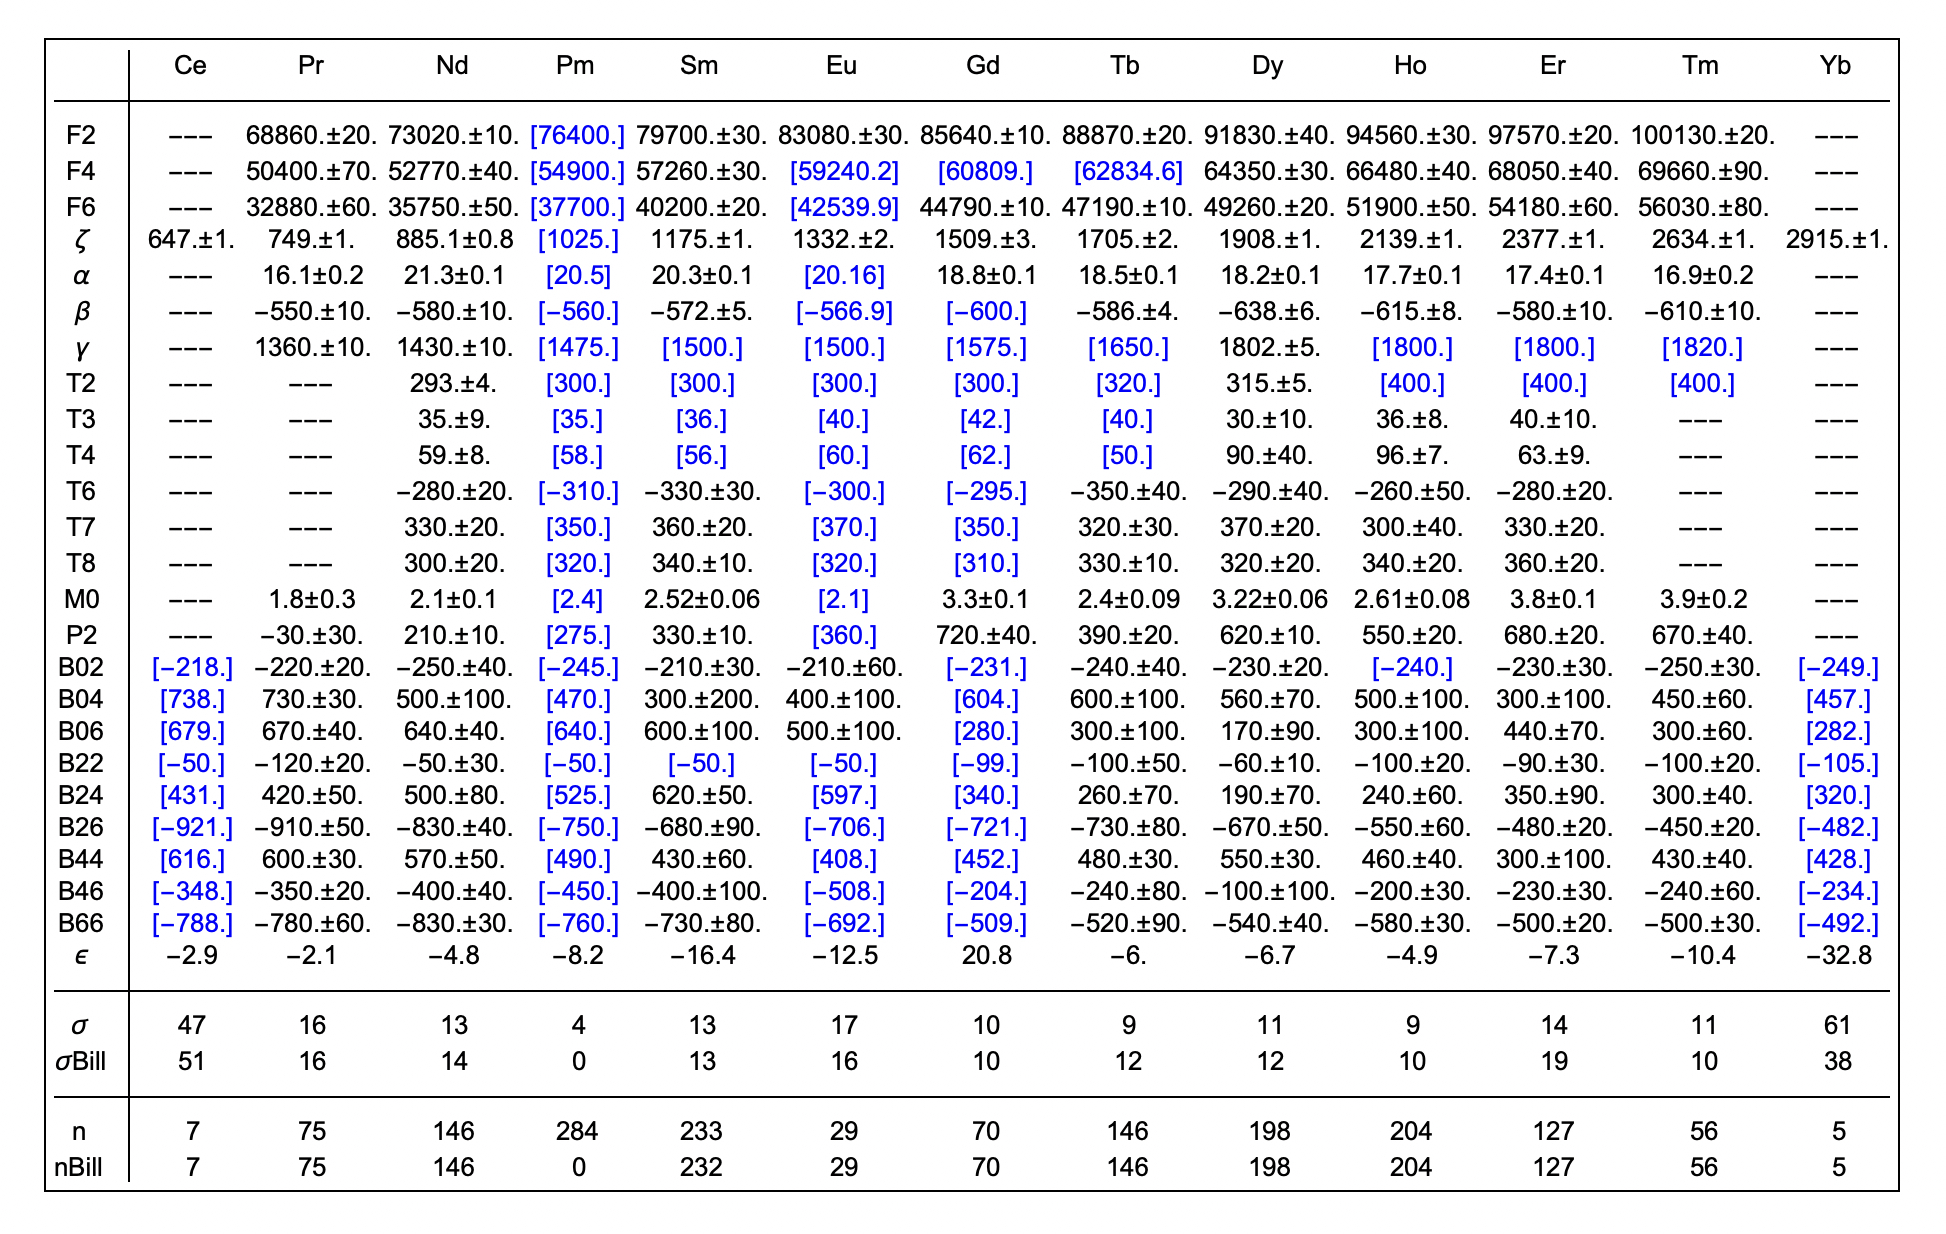
\includegraphics[width=0.95\textwidth]{fittingTable.jpg}
	\end{center}
	\caption{Fitting the data from Carnall et. al using \qlanth}
	\label{fig:refritting} 
\end{figure}

\foreach \name in {ClassicalFit}{
    \lstinputlisting[language=Mathematica]{./fundefs/\name.tex}
}

\section{Accompanying notebooks}
\qlanth is accompanied by the following auxiliary Mathematica notebooks:

\begin{itemize}
	\item \codetext{qlanth.nb}: gives an overview of the different included functions.
	\item \codetext{qlanth - Table Generator.nb}: generates the basic tables on which every calculation is based.
	\item \codetext{qlanth - JJBlock Calculator.nb}: can be used to generate the JJ blocks for the different interactions. The data files produced here are necessary for \codetext{HamMatrixAssembly} to work.
	\item \codetext{The Lanthanides in LaF3.nb}: runs \qlanth over the lanthanide ions in \LaFthree and compares the results against the published values from Carnall. It also calculates magnetic dipole transition rates and oscillator strengths.
\end{itemize}

\section{Additional data}

\subsection{Carnall et al data on Ln:\LaFthree}

The study of Carnall et al \cite{carnall_systematic_1989} on lanthanum fluoride was a systematic review of trivalent lanthanide ions in \LaFthree. In this work they fitted the experimental data for all of the lanthanide ions using the single-configuration effective Hamiltonian. In their appendices one can find their calculated values, together with the experimental values that they used for their least squares fittings. In \qlanth this data can be accessed by invoking the command \codetext{LoadCarnall} which brings into the session an Association that has keys that have as values the tables and appendices from this article. Additionally the function \codetext{LoadParameters} can be used to query the data for the fitted parameters, which may serve as a useful starting point for the description of the lanthanides ions in hosts other than \LaFthree.

\begin{figure}[htb!]
\begin{center}
	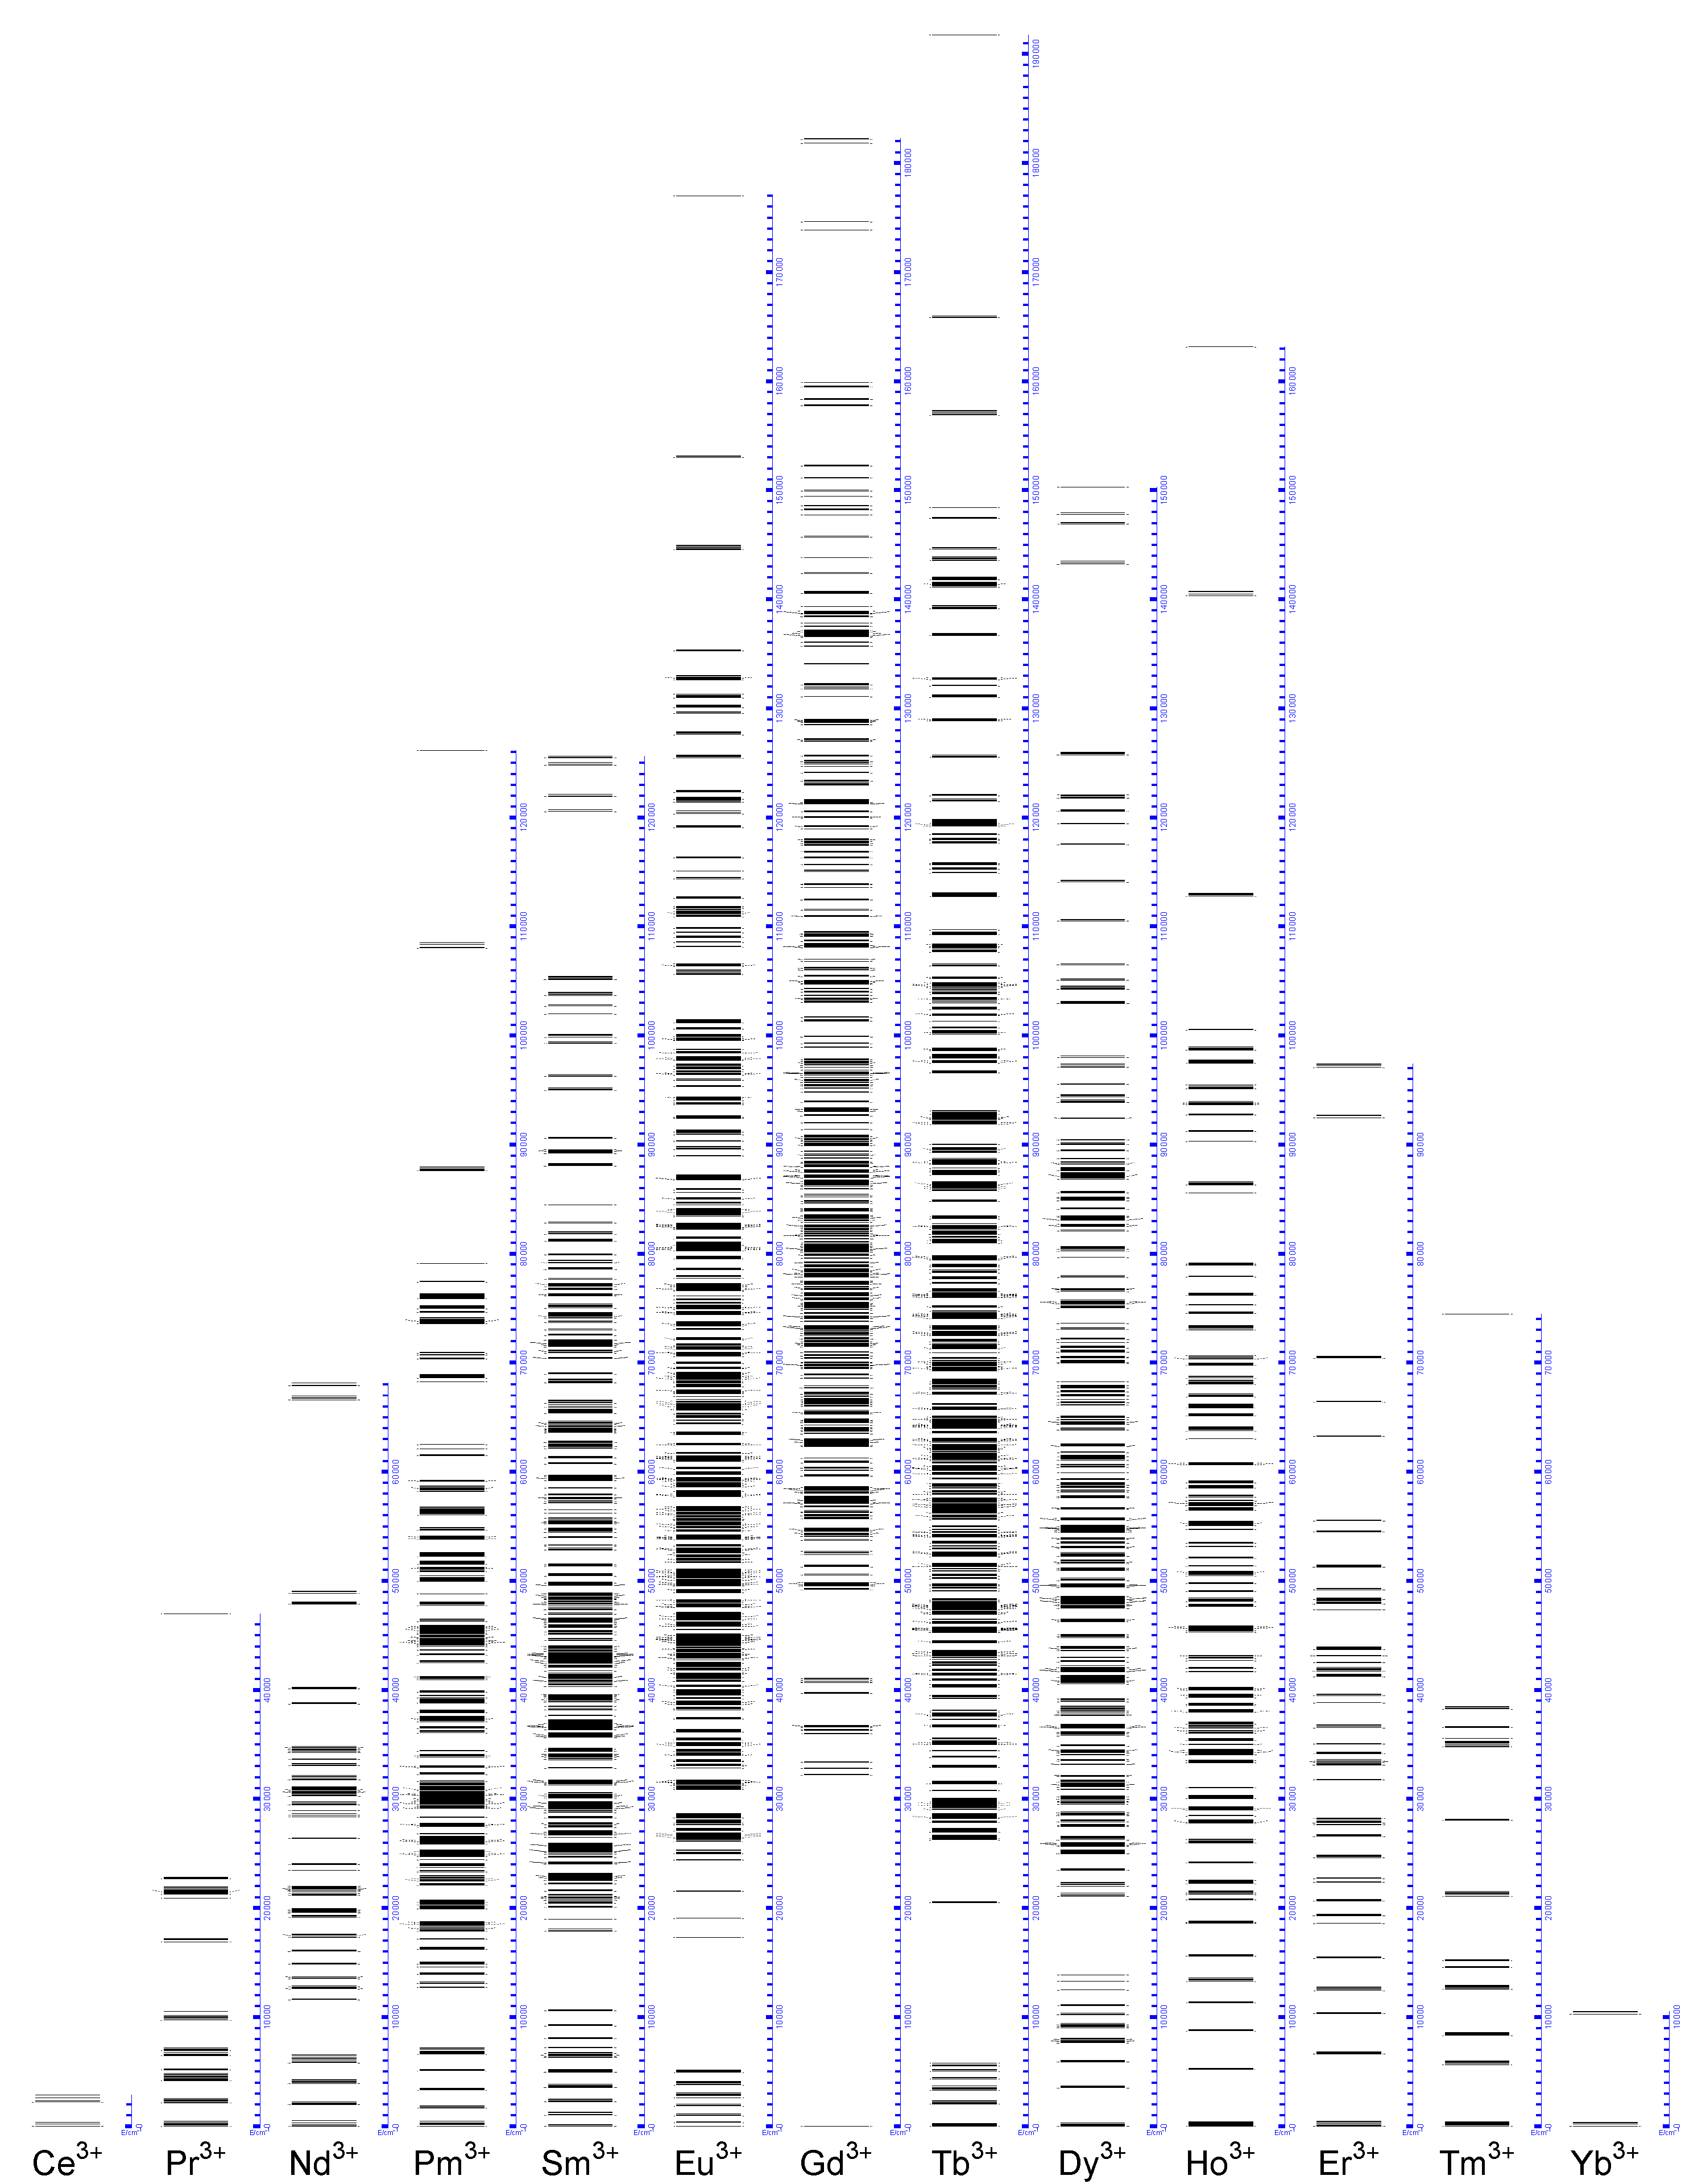
\includegraphics[width=0.99\textwidth]{DiekePlot.pdf}
\end{center}
\caption{Dieke plot for lanthanum fluoride from data generated by \qlanth.}
\end{figure}


\foreach \name in {Carnall, LoadCarnall, LoadParameters}{
    \lstinputlisting[language=Mathematica]{./fundefs/\name.tex}
}

\subsection{\codetext{sparsefn.py}}

	\qlanth is also accompanied by seven Python scripts \codetext{sparsef[1-7].py}. Each of these contains a single function \codetext{effective\_hamiltonian\_f[1-7]} which returns a sparse array for given values for the model parameters.
	
	There is an eight Python script called \codetext{basisLSJMJ.py} which contains a dictionary whose keys are f1, f2, f3, f4, f5, f6, and f7, and whose values are lists that contain the ordered basis in which the array produced by the \codetext{sparsefn.py} should be understood to be in. Each basis vector is a list with three elements \{LS string in NK notation, $J$, $\Msub{J}$\}.

	In those it is left up to the user to make the adequate change of signs in the parameters for configurations above $\forb^7$.  These include changing the signs of all in \eqnref{eqn:flipped} and setting \codetext{t2Switch} to 0. For configurations at or below $\forb^7$ it is necessary to set \codetext{t2Switch} to 1.

\section{Units}

All of the matrix elements of the Hamiltonian are calculated using the Kayser ($\text{K} \equiv \text{cm}^{-1}$) as the (pseudo) energy unit. All the parameters (except the magnetic field which is in Tesla) in the effective Hamiltonian are assumed to be in this unit. As is customary, the angular momentum operators assume atomic units in which $\hbar=1$.

Some constants and conversion values are included in the file \codetext{qonstants.m}.

\lstinputlisting[language=Mathematica]{../qonstants.m}

\section{Notation}

\begin{gather}
    \overbracket{\,\,\,\,\,\op{l}\,\,\,\,\,}^{\text{orbital angular momentum operator of a single electron}} \\
    \overbracket{\,\,\op{L}\,\,}^{\text{total orbital angular momentum  operator}} \\
    \overbracket{\,\,\op{s}\,\,}^{\text{spin angular momentum  operator of a single electron}} \\
    \overbracket{\,\,\op{S}\,\,}^{\text{total spin angular momentum operator}} \\
    \overbracket{\,\,\Lambda\,\,}^{\text{Shorthand for all other quantum numbers}} \\ 
    \overbracket{\,\,\lorb\,\,}^{\text{orbital angular momentum number}} \\
    \overbracket{\,\,\sspin\,\,}^{\text{spinning angular momentum number}} \\
    \overbracket{\,\,\CoulombNonCentral\,\,}^{\text{Coulomb non-central potential}} \\
    \overbracket{\redbraopket{\Lambda LS}{\op{O}}{\Lambda' L'S'}}^{\text{LS-reduced matrix element of operator }\hat{O}\text{ between }{\Lambda LS} \text{ and } {\Lambda' L'S'}} \\
    \overbracket{\redbraopket{\Lambda LSJ}{\op{O}}{\Lambda' L'S'J'}}^{\text{LSJ-reduced matrix element of operator }\hat{O}\text{ between }{\Lambda LSJ} \text{ and } {\Lambda' L'S'J'}} \\
    \overbracket{\LSterm{2 S + 1}{\alpha{L}}\equiv \ket{\alpha{LS}}}^{\text{Spectroscopic term } {\alpha{LS}} \text{ in Russel-Saunders notation }} \\
    \overbracket{\op{X}^{(k)}}^{\text{spherical tensor operator of rank k}} \\
    \overbracket{\op{X}_q^{(k)}}^{\text{q-component of the spherical tensor operator }\op{X}^{(k)}} \\
    \overbracket{\cfp{\lorb^{n-1}\alpha'L'S'}{\lorb^n\alpha{L}{S}}}^{\text{The coefficient of fractional parentage from the parent term }\ket{\lorb^{n-1}\alpha'{L'S'}}\text{ for the daughter term }\ket{\lorb^{n}\alpha{LS}}}  
\end{gather}



\section{Definitions}  

\begin{gather} 
    \overbracket{\tpobraket{x} \DEF 2x+1}^{\text{two plus one}} \\
    \overbracket{\op{u}^{(k)}}^{\text{irreducible unit tensor operator of rank k}} \\ 
    \overbracket{\op{U}^{(k)} \DEF \sum_{i=1}^{n} \op{u}^{(k)} }^{\text{symmetric unit tensor operator for n equivalent electrons}} \\
    \overbracket{\Ckq{k}{q} \DEF \sqrt{\frac{4\pi}{2k+1}} \Ykq}^{\text{Renormalized spherical harmonics}} \\
    \overbracket{\tricondition{j_1,j_2,j_3} \DEF
    \begin{cases} 
        1 & \text{if } j_1 = (j_2 + j_3), (j_2 + j_3 - 1), \ldots, |j_2-j_3|\\
        0 & \text{otherwise}
        \end{cases}}^{\text{Triangle ``delta'' between $j_1,j_2,j_3$}} 
\end{gather}

\newpage

\section{code}

\subsection{qlanth.m}

This file encapsulates the main functions in \qlanth and contains all the Physics related functions.

\lstinputlisting[language=Mathematica]{../qlanth.m}

\subsection{fittings.m} 

This file has code useful for fitting the Hamiltonian.

\lstinputlisting[language=Mathematica]{../fittings.m}

\subsection{qonstants.m} 

This file has a few constants and conversion factors.

\lstinputlisting[language=Mathematica]{../qonstants.m}

\subsection{qplotter.m}

This module has a few useful plotting routines.

\lstinputlisting[language=Mathematica]{../qplotter.m}

\subsection{misc.m}

This module includes a few functions useful for data-handling.

\lstinputlisting[language=Mathematica]{../misc.m}

\subsection{qalculations.m}

This script encapsulates example calculations in which the level structure and magnetic dipole transitions are calculated for the lanthanide ions in lanthanum fluoride.

\lstinputlisting[language=Mathematica]{../qalculations.m}

\newpage

\printbibliography

\end{document} 
